\chapter{\label{ch:4-microboone}The MicroBooNE experiment}

\minitoc


This chapter presents an overview of the MicroBooNE experiment, with a focus on the Liquid Argon Time Projection Chamber technology. A description of the MicroBooNE detector is essential in order to understand the analysis described in the following chapters. The selection efficiency of low-energy electron neutrino events and the rejection of background events can directly depend on the detector properties. The analysis is also affected by systematic uncertainties in the detector simulation, which will be partially addressed here. A brief description of the MicroBooNE neutrino beam will also be provided.

\section{Motivation}
The MicroBooNE (Micro Booster Neutrino Experiment) experiment is an 89~t active volume Liquid Argon Time Projection Chamber (LArTPC) located at the Fermi National Accelerator Laboratory (FNAL) in Batavia, IL and on-axis with the Booster Neutrino Beam (BNB). The experiment was designed to study short-baseline neutrino oscillations and neutrino-argon cross section. It is the largest neutrino LArTPC detector currently active in the world.
This technology offers very high spatial resolution and calorimetric capabilities, which allow for detailed tracking, vertexing, and particle identification. 

\subsection{Physics goals}
As described in Section \ref{sec:miniboone}, MiniBooNE, being a Cherenkov detector, is not able to distinguish between single photons and electrons in the final state. As such, it is not possible to determine the nature of the excess of low-energy events. If the excess is caused by photons, one explanation could be provided by an underestimation of one of the background components. An electron nature of the excess, instead, could be a strong hint for BSM physics.

\subsubsection{Addressing the MiniBooNE anomaly}
The MicroBooNE experiment was designed to definitely clarify the MiniBooNE anomaly since the LArTPC technology allows for powerful electron/photon separation. One way to achieve this goal is to measure the spatial gap between the neutrino interaction vertex and the start of the electromagnetic shower. An electron will start producing a ionising trail immediately, whereas a photon will usually leave a visible gap, due to the radiation length in liquid argon $X_0 = 14$~cm.
A second way to distinguish between electrons and photons is to measure the energy loss per distance travelled ($dE/dx$) of the electromagnetic shower produced in the liquid argon. For electrons above 100~MeV, the theoretical expectation of the most probable $dE/dx$ is around 2~MeV/cm, while the photon will have a most probable value approximately twice as large, due to the pair-production process $\gamma\rightarrow e^+e^-$ \cite{Acciarri:2016sli}. 
MicroBooNE is then performing two parallel analyses, one assuming that the excess is caused by photon production in the electromagnetic $\Delta\rightarrow N\gamma$ decay and one assuming that the excess is caused by electron interactions. The calorimetric and spatial-resolution capabilities will allow having a sensitivity to the excess similar to MiniBooNE, while having an active detector mass five times smaller.  The search for electron-like low-energy interactions will be described in detail in the following chapters.

\subsubsection{Cross-section measurements}
MicroBooNE will also provide precise neutrino-nucleon cross-section measurements. The neutrino interactions in the energy range of the BNB span from quasi-elastic to deep inelastic scattering, making it possible to explore several nuclear effects and complex topologies.
In particular, it is possible to measure the pion production in neutral current (NC) and charged current (CC) interactions. MicroBooNE should be able to solve the tension between the large NC $\pi^0$ component reported by MiniBooNE \cite{AguilarArevalo:2008xs} and the small CC $\pi^+$ component reported by SciBooNE \cite{Hiraide:2008eu} and K2K \cite{Tanaka:2006zm}. 
A precise measurement of the photon production will also help to constrain the $\Delta\rightarrow N\gamma$ background, important for the MiniBooNE low-energy excess analysis. 

The measurement of neutrino cross sections in liquid argon is also of fundamental importance for the design of the largest next-generation neutrino experiment, DUNE (Deep Underground Neutrino Experiment). Its current proposed design includes a 40-kton LArTPC as far detector, two orders of magnitude larger than MicroBooNE \cite{Acciarri:2016ooe}.

\subsubsection{Supernova and exotic searches}
The MicroBooNE detector is located just below the surface level and is constantly bombarded by cosmic rays, which interact in the liquid argon leaving ionisation trails. This background, together with the small active volume of the detector (compared with large-scale water Cherenkov experiments) can limit the capabilities of certain physics analyses, such as proton decay searches. However, MicroBooNE can study the interaction of charged kaons in the liquid argon, which can represent a background to future proton decay searches in DUNE.
The existence of proton decay is predicted by several Grand Unification Theories (GUTs) and a lower proton lifetime of $5.9\times10^{33}$ years was set by the Super-Kamiokande experiment looking at the $p\rightarrow \nu K^+$ \cite{Abe:2014mwa}. The kaon decay chain $K\rightarrow\pi\rightarrow\mu\rightarrow e$ represents also an important benchmark for the reconstruction capabilities of the LArTPC.

The MicroBooNE detector is suited to detect neutrinos produced by a supernova (SN) in the Milky Way or in its immediate surroundings, which would result in around 30 CC $\nu_e$ interactions with electron energy above 10~MeV. However, being constantly hit by cosmic rays, the detector cannot directly trigger on SN neutrinos and it relies on the SuperNova Early Warning System (SNEWS) \cite{Antonioli:2004zb} to record an eventual SN event. 


\subsection{Research and development goals}
MicroBooNE is currently the largest active neutrino LArTPC in the world, which makes it the first experiment to precisely assess the automated neutrino reconstruction capabilities of this technology. The detection of neutrinos by a large-scale LArTPC was pioneered by the ICARUS collaboration, which designed and assembled the ICARUS T600 detector \cite{Amerio:2004ze}. The detector consists of two LArTPC modules with a total active mass of 476~t, around five times larger than MicroBooNE. However, it was employed as a long-baseline neutrino detector on the CNGS (CERN Neutrinos to Gran Sasso) beam and it detected only four $\nu_e$ interactions \cite{Antonello:2013gut}, compared with the several hundred expected at MicroBooNE. It was recently refurbished and moved to Fermilab to be placed on the BNB, as a part of the future Short Baseline Neutrino (SBN) program. On a smaller scale, the ArgoNeuT experiment operated a 0.25~t TPC on the NuMI neutrino beam at Fermilab \cite{Anderson:2012vc} and measured for the first time the neutrino cross section on argon atoms.

The ambitious physics program of the DUNE experiment, whose ultimate goal is to verify the presence of CP violation in the leptonic sector, requires a very good understanding of the technology: in particular, the effect of high electric field on long distances, of the ions recombination in the LAr, and of the ions absorption by the impurities must be precisely quantified. 
MicroBooNE was also the first large-scale LArTPC to have part of the electronics chain operating directly in the liquid argon (\emph{cold electronics}), allowing for higher signal-to-noise ratio. An overview of the MicroBooNE detector will be provided in Section \ref{sec:detector}.
A small-scale prototype of the DUNE detector, ProtoDUNE, was recently built and commissioned at CERN, with an active mass of 450~t. The ProtoDUNE detector, however, runs on a test-beam line and will not detect neutrino interactions.

\section{The LArTPC detection technology}
The concept of a Liquid Argon Time Projection Chamber was first laid out by Willis and Radeka in 1974 \cite{Willis:1974gi} and then adapted by Rubbia in 1977 as a detector for neutrino interactions \cite{Rubbia:1977zz}. 

Generally speaking, a Time Projection Chamber is a volume with a constant electric field applied between two of its sides, the anode (the positive plane) and the cathode (the negative plane). It is possible to fill the volume with a non-conductive material such as inert gases or liquids. %A magnetic field can also be applied to measure the charge and the momentum of the particle interacting in the TPC (it is not the case of MicroBooNE). 

A charged particle traversing the medium inside the TPC will ionise the material: a trail of ionisation electrons will be produced in correspondence with the path of the charged particle. The constant electric field will transport the electrons towards the anode with a constant drift velocity, preserving their topological and calorimetric information and appearing as a projection of the particle trajectory on the anode plane. The distance between the anode and the interaction point will be given by the time the ionisation electron takes to reach the anode. Figure \ref{fig:lartpc_diagram} shows the operating principle of a TPC in the case of the MicroBooNE detector. 

\begin{figure}[htbp]
    \centering
    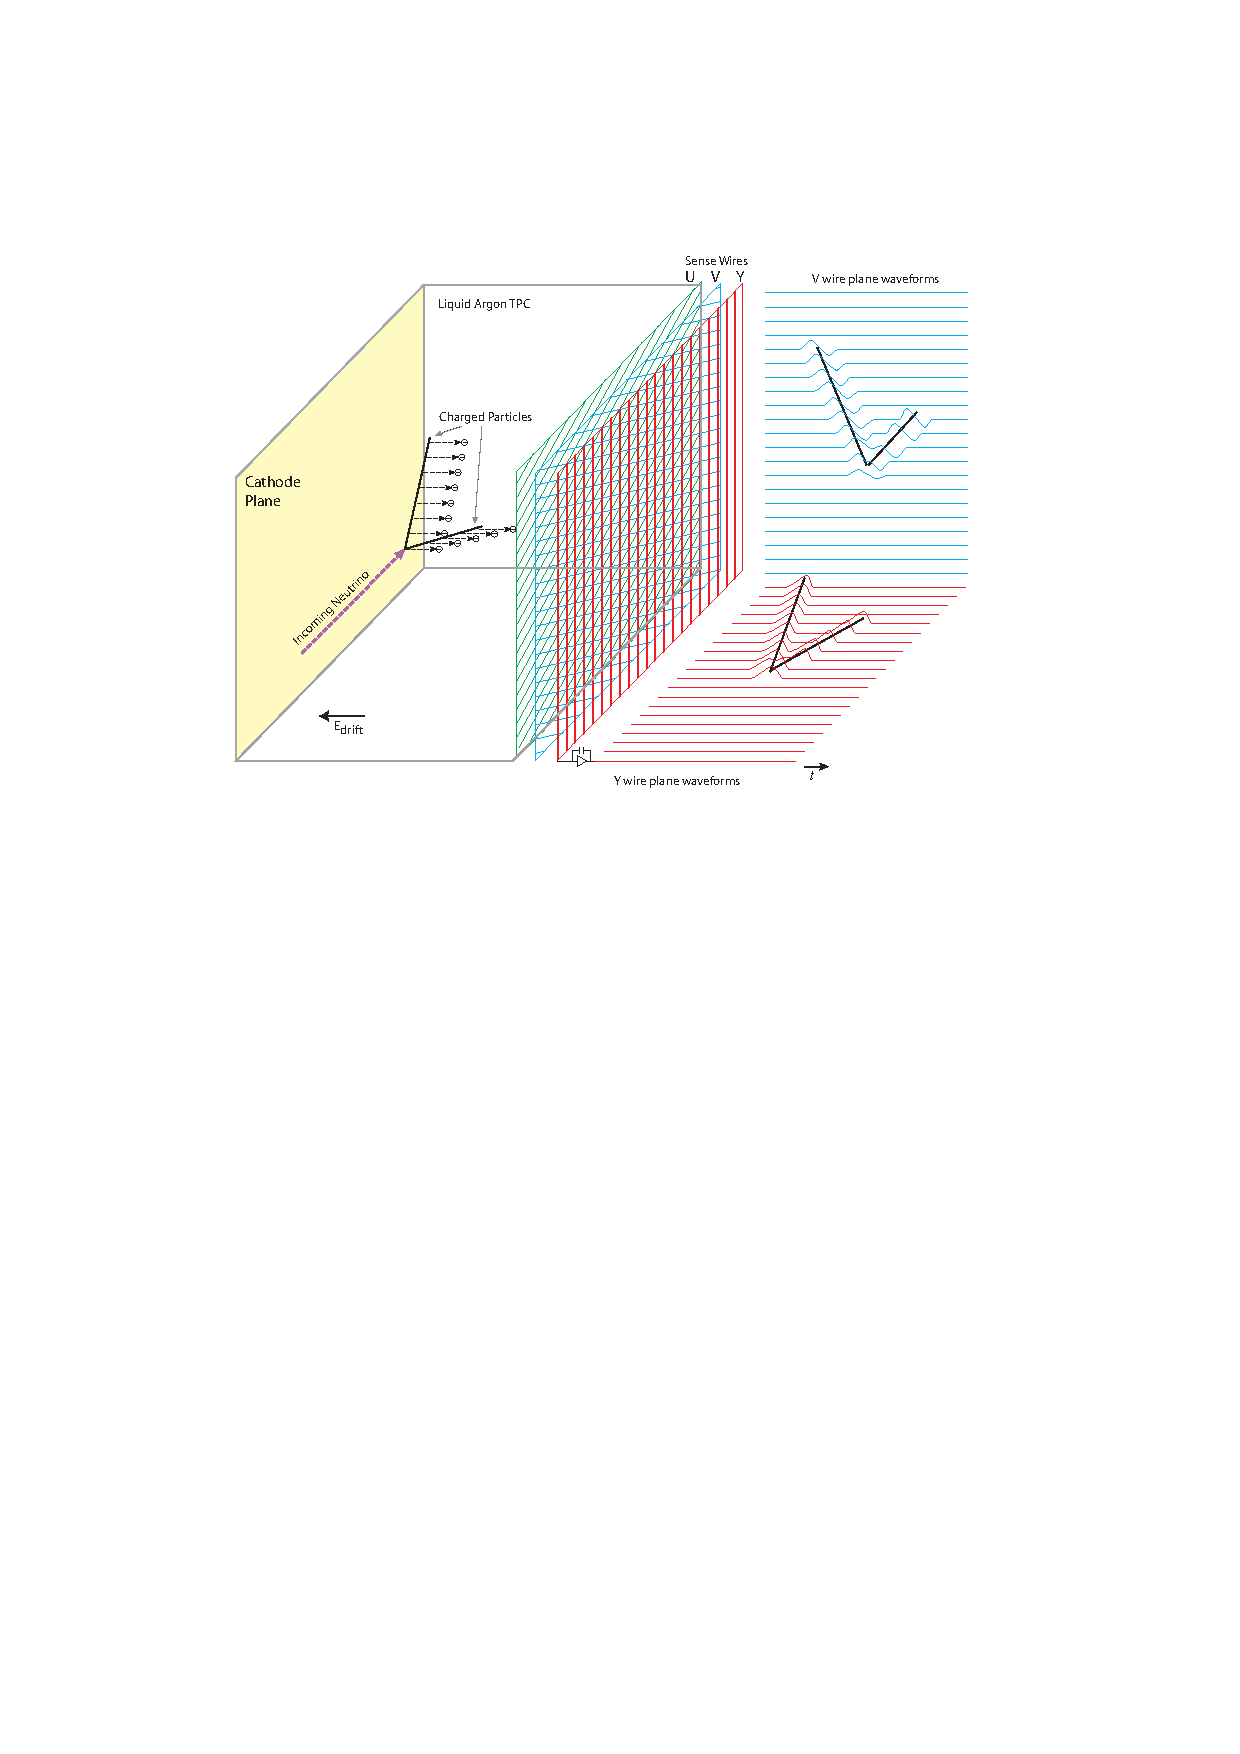
\includegraphics[width=0.8\linewidth]{figures/lartpc_diagram.pdf}
    \caption{Diagram of the operating principle of the MicroBooNE LArTPC, showing the waveforms produced by the ionisation trails in the collection plane (red) and in one induction plane (blue).}
    \label{fig:lartpc_diagram}
\end{figure}

As the name says, a LArTPC is a TPC filled with liquid argon. This material provides several advantages, which made this technology particularly suitable for neutrino detection. Among the main ones we can enumerate (1) its substantial density (1.4~g/cm$^3$ at 87.3~K), which allows to have a detectable amount of neutrino interactions, (2) its high stability, being a noble gas, and (3) its natural abundance (1\% of the atmosphere), which makes the LArTPC technology highly scalable and affordable.

However, the relatively slow drift velocity of the electrons in the liquid argon causes the typical read-out of a large-scale LArTPC to be in the order of the milliseconds (which corresponds to the time a ionisation electron takes to travel from the cathode to the anode), making this technology sub-optimal for high-rate experiments. 

Another fundamental property of the argon, which makes it particularly suitable for high-energy physics experiments, is that it produces scintillation light when excited, being at the same time transparent to the wavelength of this scintillation light, described below. In this way, a detector on surface such as MicroBooNE can collect the light (in our case with photomultipliers placed inside the LAr) and trigger the TPC readout in coincidence with the neutrino beam, suppressing the background caused by cosmic rays outside the beam time window. 

A LArTPC can achieve a very high spatial resolution, similar to the one of the bubble chambers, allowing at the same time for the digitisation of the signal. For this reason, it has often been called a \emph{fully electronic bubble chamber} \cite{Rubbia:2011zza}. 

\subsubsection{Light production}
The scintillation light is produced when an atom of argon in the ground state shares an electron with one argon of atom in an excited state, forming an Ar$_{2}$ \emph{excimer}. When the excimer decays and a 128~nm photon is emitted, the two argon atoms are both left in the ground state. This small wavelength is typically difficult to detect with standard photomultipliers. In the MicroBooNE experiment, the PMT plates are coated with tetraphenyl butadiene (TPB), which acts as wavelength shifter. The time distribution of the scintillation light emission has two characteristics components at 6~ns and 1.5 \si{\micro}s.

The liquid argon has also a high light yield, comparable to the one of scintillating crystals, with $4\times10^4$~$\gamma$/MeV. The amount of light, however, can be quenched by the presence of nitrogen impurities in the argon, which, in the case of MicroBooNE, are kept below the 2~ppm level.

\subsubsection{Ionisation electrons}\label{sec:ionisation}
The work function for ionising an argon atom is $W_{\mathrm{ion}} = 23.6$~eV, which means that a charged particle in the MeV range will leave a ionisation trail of tens of thousands of electrons. Under an electric field, these free electrons will travel towards the anode with a constant drift velocity, but during their path they can undergo several attenuation processes, which decrease the actual number of electrons reaching the wire plane. 

In particular, the electrons can recombine with ionised Ar$^+$ atoms: this recombination effect is usually the main contributor to the signal attenuation. This effect depends on the $dE/dx$ of the particle, on the electric field in the liquid argon, and on the angle of the ionisation particle with respect to the electric field. The ICARUS experiment measured the dependence of the recombination as a function of the $dE/dx$ and the applied electric field \cite{Amoruso:2004dy}, as shown in Figure \ref{fig:recombination}. The ArgoNeuT experiment found the recombination effect in a LArTPC to be well described both by the Birks' model \cite{Birks:1951boa} and by a modified version of the Box model \cite{Thomas:1987zz}. 

\begin{figure}[htbp]
\centering
  \begin{subfigure}{0.48\textwidth}
    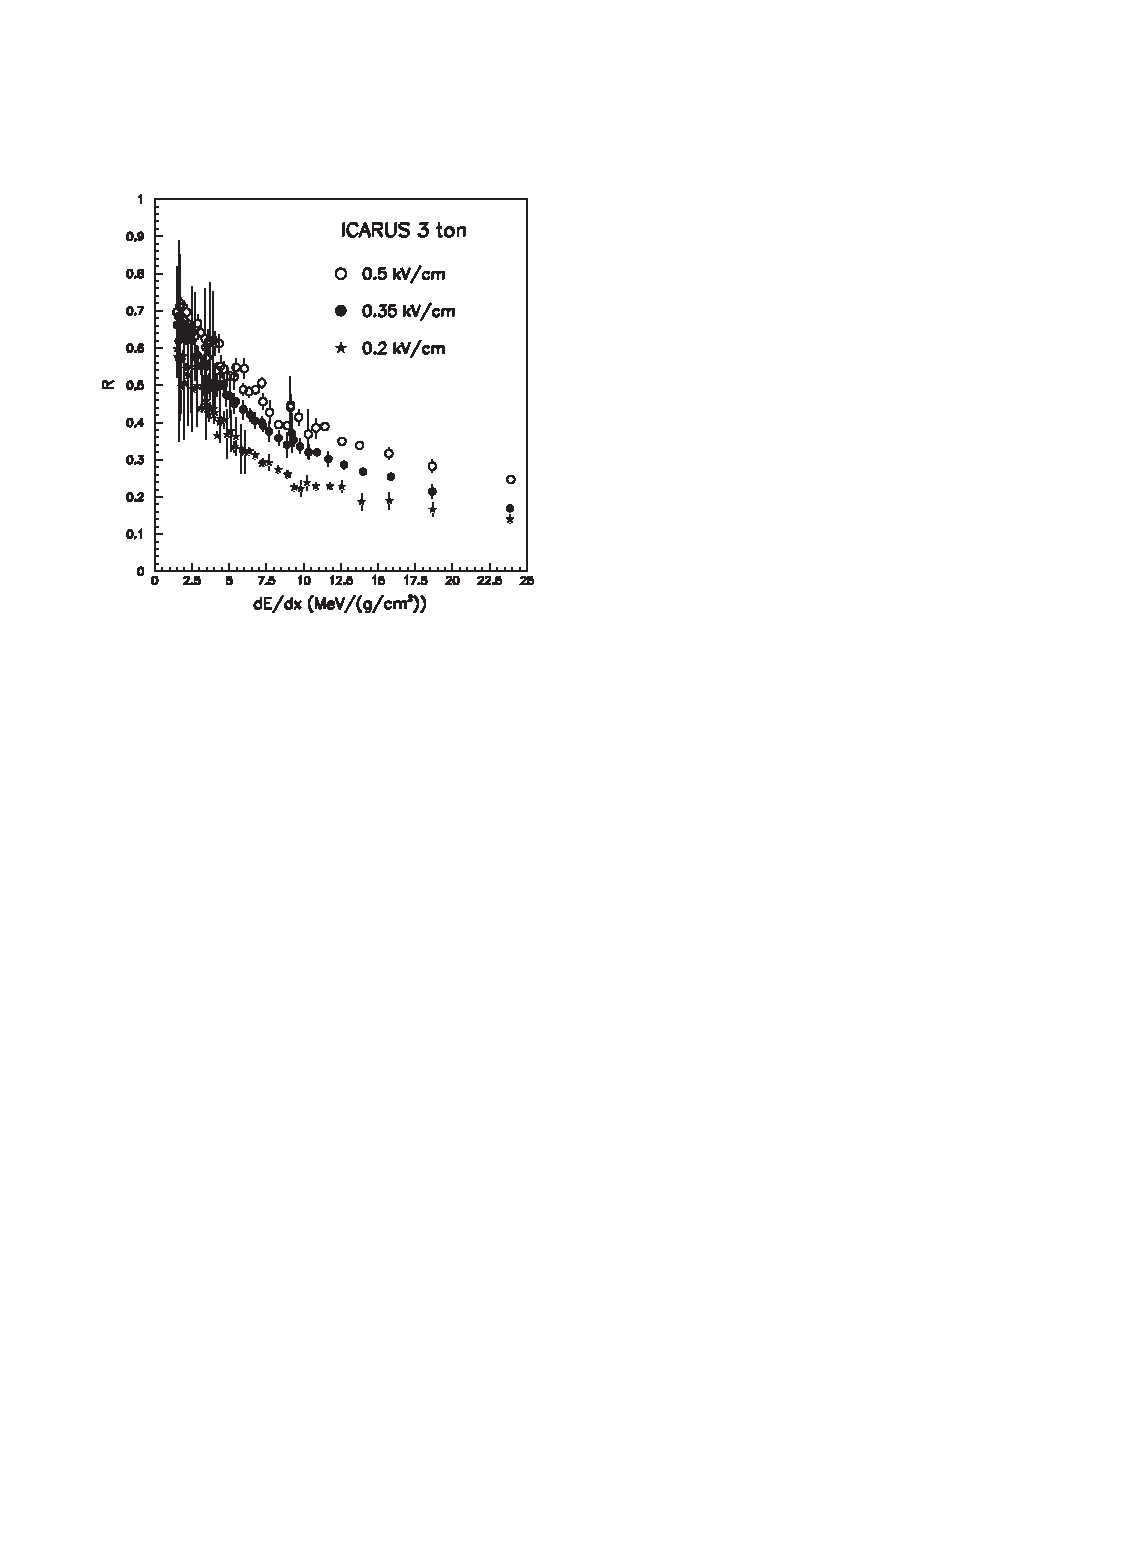
\includegraphics[height=0.9\linewidth]{figures/icarus1.pdf}
    \caption{Recombination factor as a function of the particle $dE/dx$.}
  \end{subfigure}\hfill
  \begin{subfigure}{0.48\textwidth}
    \begin{center}
        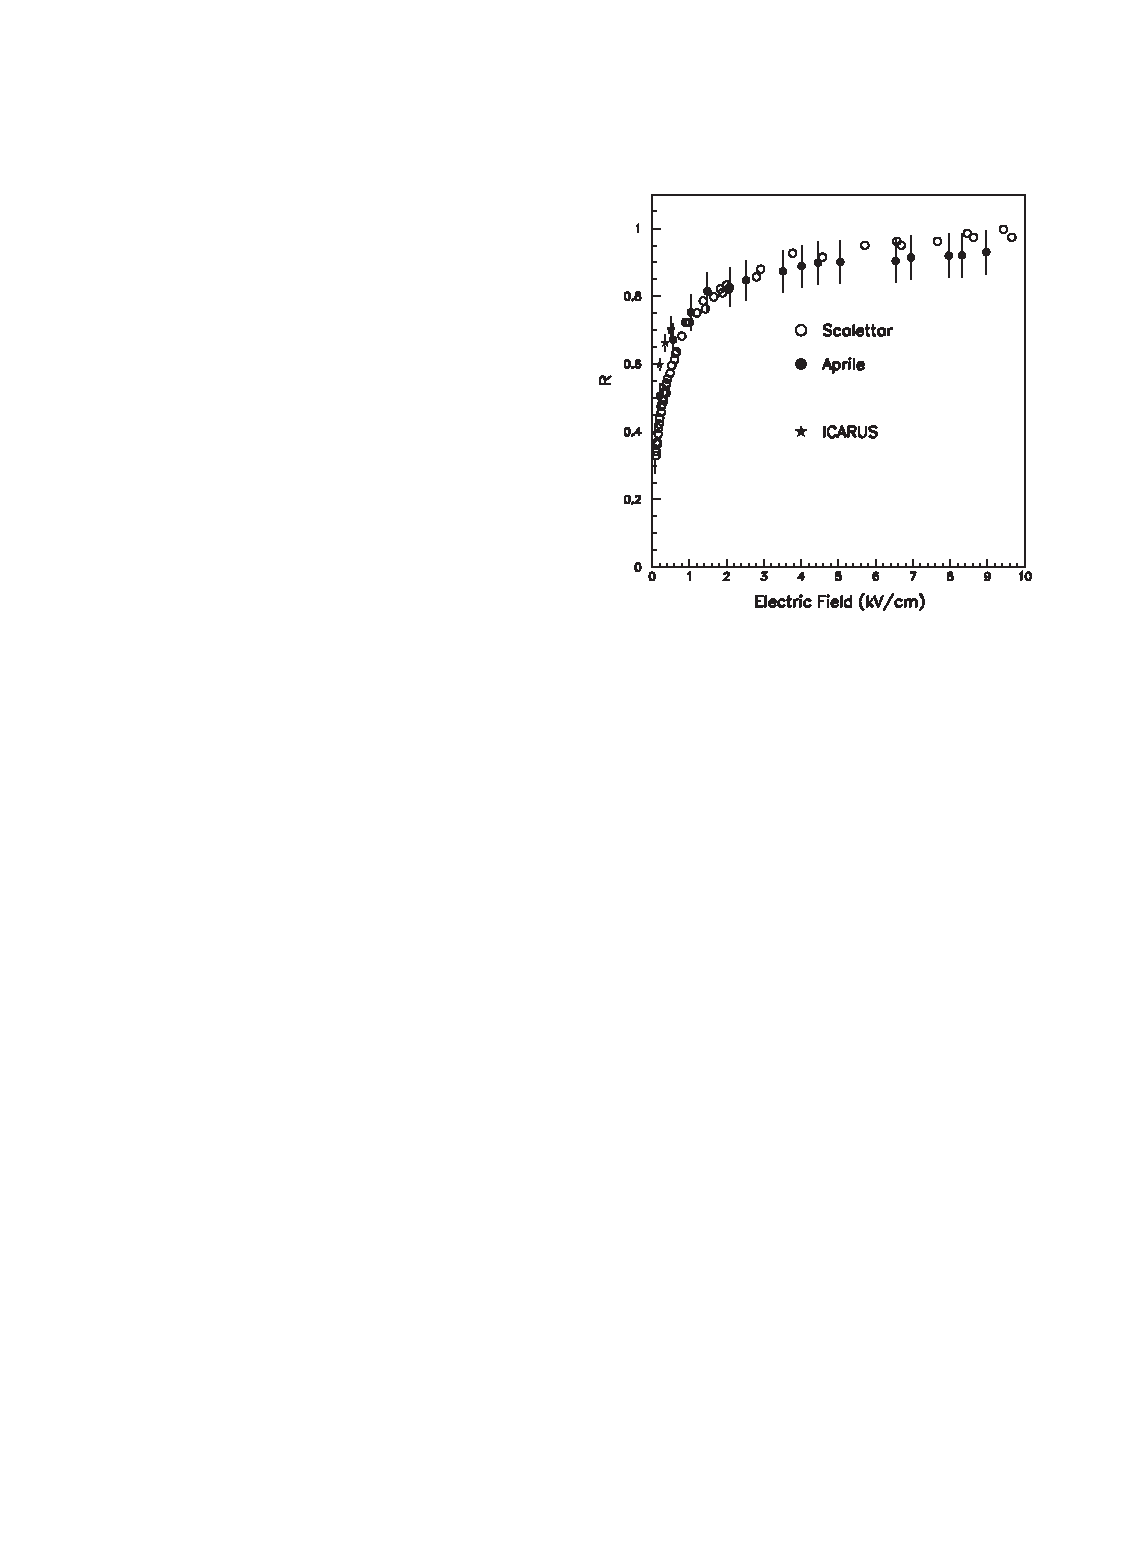
\includegraphics[height=0.9\linewidth]{figures/icarus2.pdf}
        \caption{Recombination factor as a function of the electric field in the detector.}
    \end{center}
  \end{subfigure}
    \caption{The ICARUS collaboration measured the recombination factor \emph{R}, defined as the ratio between the measured and the theoretical stopping power, as a function of the $dE/dx$ (left) and of the electric field (right). From \cite{Amoruso:2004dy}.}\label{fig:recombination}
\end{figure}

The transport of the electrons in the LArTPC is affected by diffusion, caused by their thermal velocity, which spreads out the ionisation electrons while they travel towards the anode. It is a three-dimensional effect, usually separated into its longitudinal and transverse components. 

LArTPCs placed on surface, such as MicroBooNE, are also constantly hit by an intense flux of cosmic rays, which will produce several ionisation trails. These trails produce ionisation electrons and positive Ar$^+$, with the ions slowly moving towards the cathode until they will recombine with a free electron. The build-up of Ar$^+$ ions leads to a distortion of the electric
field within the detector, defined as \emph{space-charge effect} (SCE). The SCE causes a displacement in the reconstructed position of ionisation electrons, as well as variations in the amount of charge quenching experienced by ionisation throughout the volume of the TPC. In MicroBooNE, the electric field distortion can be as high as 15\% and was measured using a sample of cosmic rays triggered by a small cosmic-ray counter (briefly described in Section \ref{sec:crt}) \cite{sce}. The spatial distortions at the top and the bottom of the LArTPC are shown in Figure \ref{fig:spacecharge}.

\begin{figure}[htbp]
    \centering
    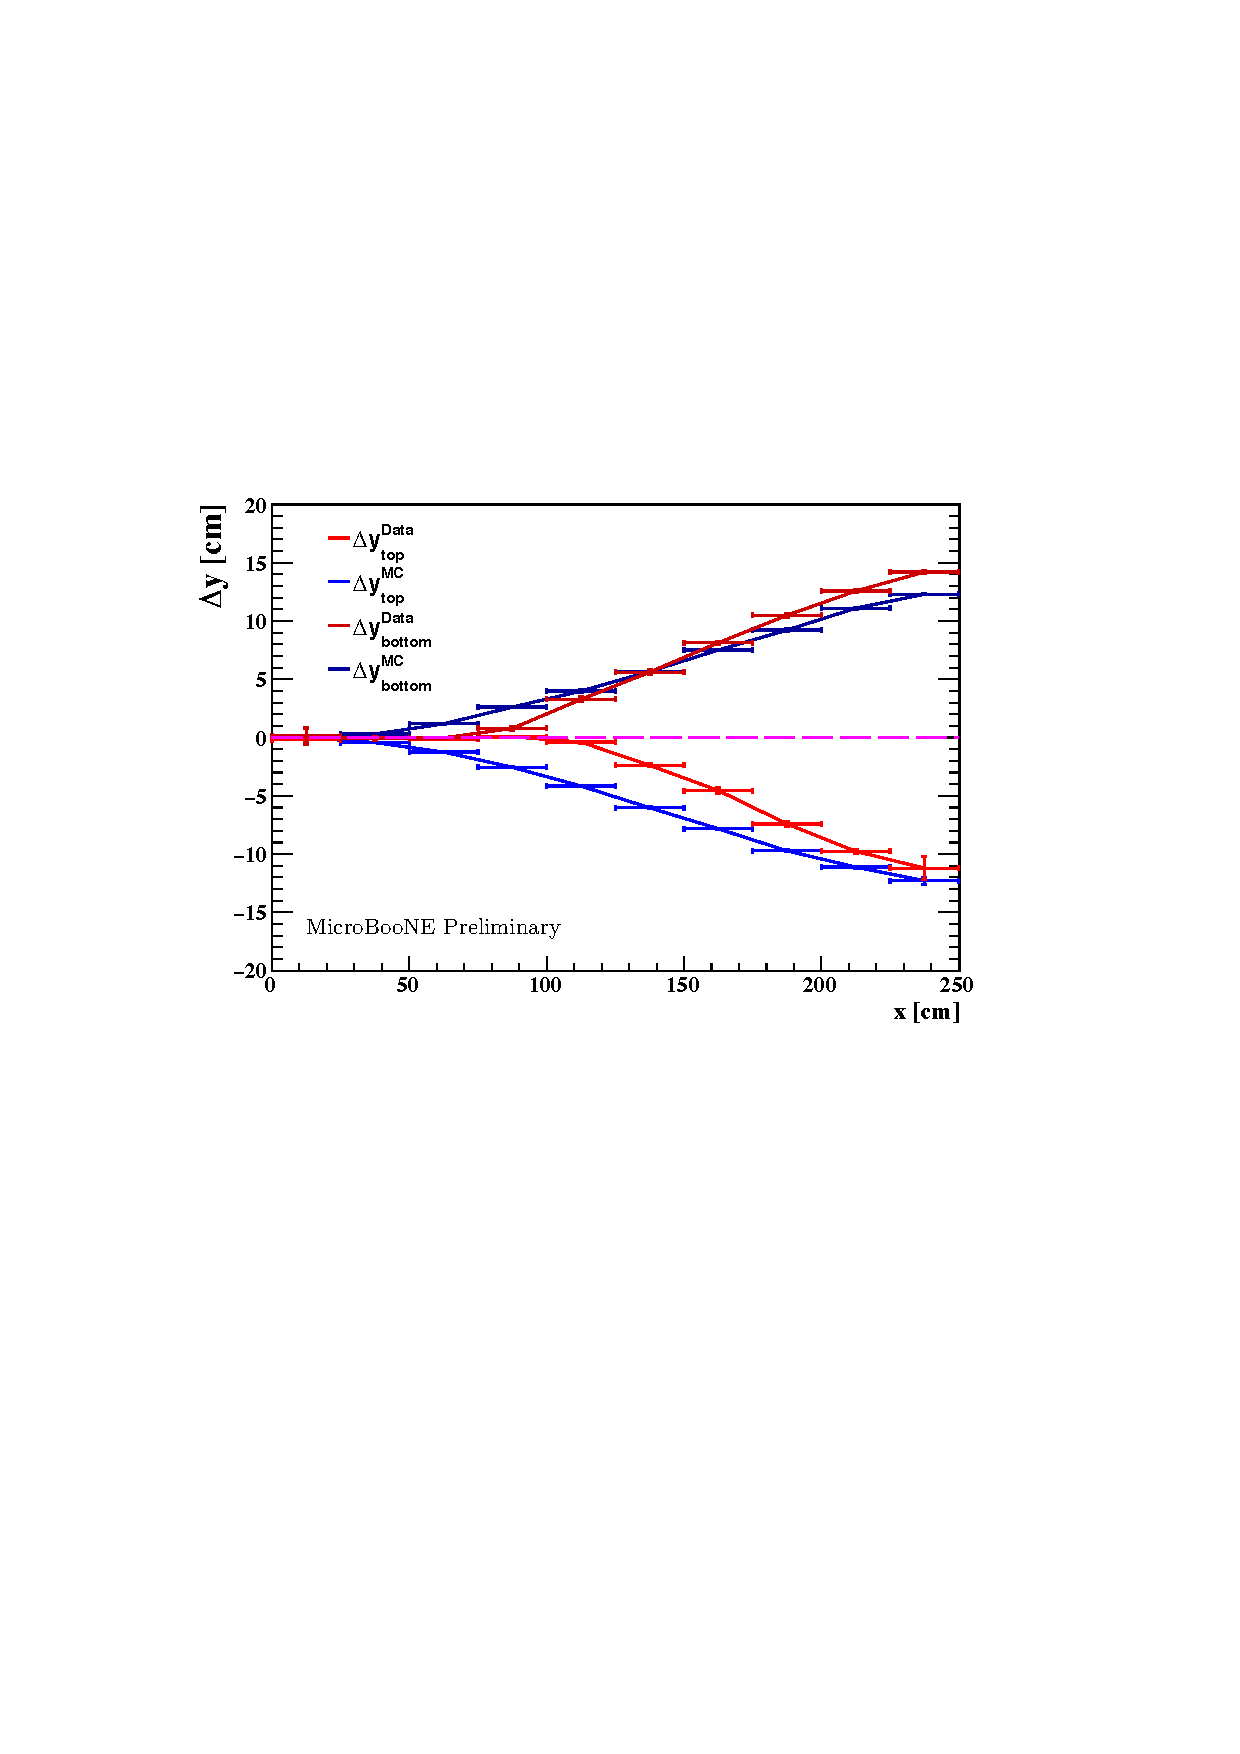
\includegraphics[width=0.8\linewidth]{figures/spacecharge.pdf}
    \caption{Predicted ($\Delta y^{\mathrm{MC}}$) and measured ($\Delta y^{\mathrm{Data}}$) space-charge distortions as a function of the drift coordinate at both the top and bottom of the TPC. The discrepancy between data and Monte Carlo is caused by the absence of the liquid argon flow in the simulation. Error bars are statistical only. From \cite{sce}.}
    \label{fig:spacecharge}
\end{figure}

The presence of impurities in the liquid argon, such as oxygen, nitrogen, and water can also attenuate the signal, absorbing the ionisation electrons during their path in the liquid argon. The amount of drifting electrons decline as a function of the distance from the wire plane, since the electrons need to travel a longer path. The attenuation is well modelled by an inverse exponential function and the decay time constant is called \emph{electron lifetime}. MicroBooNE purification system, described in Section \ref{sec:detector}, achieved an O$_2$ contamination smaller than 100~ppt and an electron lifetime larger than 18~ms \cite{Meddage:2017lxo}. In MicroBooNE, the electron lifetime was estimated by measuring the ratio between the charge at the anode and the charge at the cathode with crossing cosmic muons, through the relation:
\begin{equation}
    \frac{Q_A}{Q_C} = \exp(-t_{\mathrm{drift}}/\tau),
\end{equation}
where $t_\mathrm{drift}$ is the drift time (2.3~ms) and $\tau$ is the electron lifetime. Figure \ref{fig:purity} shows the variation of the $Q_A/Q_C$ ratio over time in the MicroBooNE LArTPC.

\begin{figure}[htbp]
    \centering
    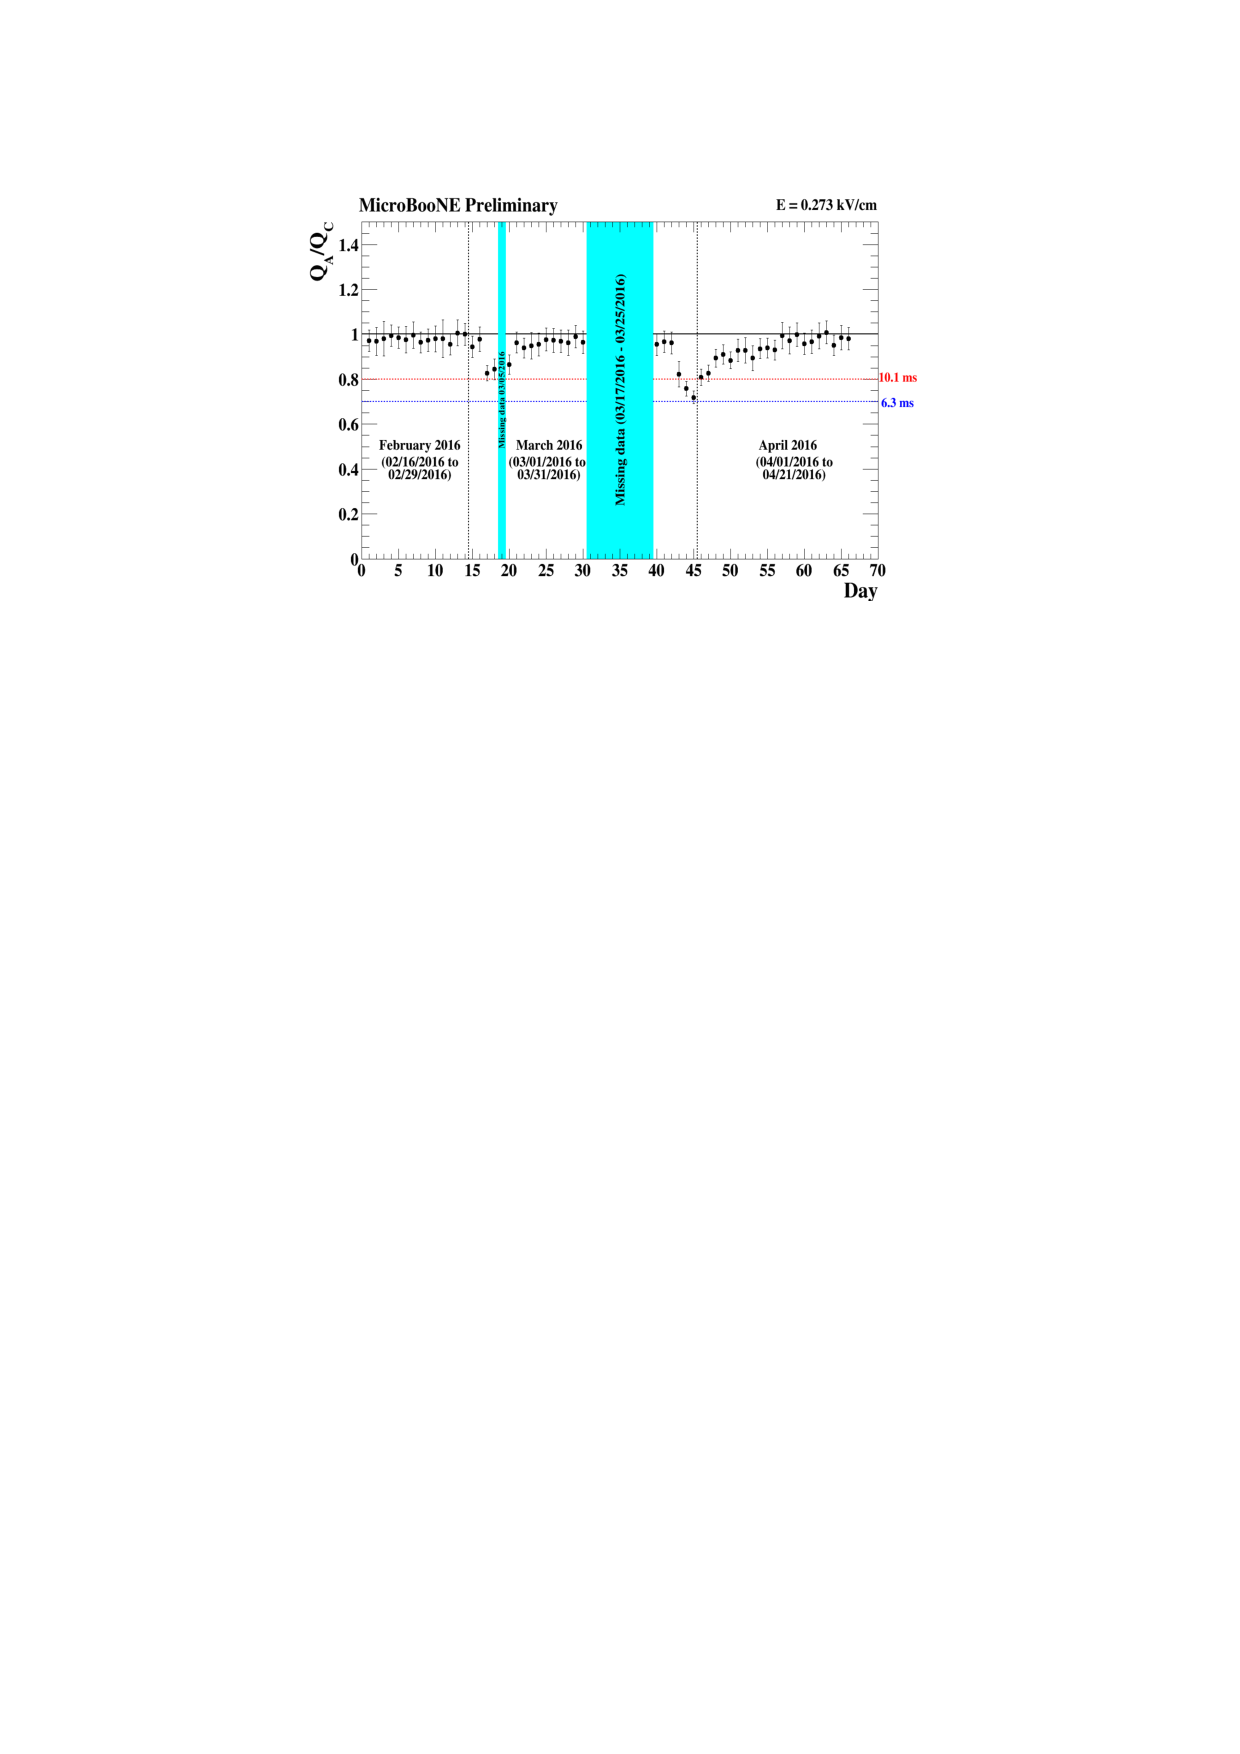
\includegraphics[width=0.7\linewidth]{figures/purity.pdf}
    \caption{Variation of the $Q_A/Q_C$ charge ratio between February and April 2016 in the MicroBooNE LArTPC. From \cite{Meddage:2017lxo}.}
    \label{fig:purity}
\end{figure}
 
\section{The neutrino beams at Fermilab}\label{sec:beam}
The use of an artificial neutrino source presents two main advantages: (1) the neutrino energy spectrum and its flavour components can be precisely characterised and tuned for the specific physics goals, and (2) the position of the detector can be optimised to observe the oscillation peak (or dip). The design of a neutrino beam generally follows the same pattern: it starts with a proton beam, which hits a target and produces hadrons. These hadrons are focused by a magnetic horn into an empty pipe, where they decay, producing the neutrinos. The neutrino beam then travels through the ground and hits one or more neutrino detectors.

At Fermilab, there are two neutrino beams currently active: the Booster Neutrino Beam (BNB) and the Neutrinos from the Main Injector (NuMI) beam, with different energy, flavour composition, and direction. MicroBooNE is placed on-axis with the BNB and 470~m far from the target. While it is also able to detect off-axis neutrinos from the NuMI beam, the analysis presented in this document will focus on the neutrinos coming from the BNB.

The accelerator chain starts with a source of hydrogen gas, which is ionised and accelerated by an empty cavity with -35~kV voltage. This H$^-$ stream is focused by two solenoids and transformed into a pulsed beam 100~\si{\micro}s long at 15~Hz. The Radio Frequency Quadrupole (RFQ) then accelerates the beam to an energy of 750~keV. The H$^-$ beam is then fed to the Linear Accelerator (LINAC), where two series of RF cavities bring it from 750 keV to 400~MeV.  The negative hydrogen ions are stripped of their electrons by a carbon foil and the proton beam is finally injected into the Booster synchrotron. Here, after several thousand laps, the proton beam reaches their maximum kinetic energy in the Booster of 8~GeV.

The 8~GeV proton batch is 1.6~\si{\micro\second} long and divided into 84 bunches 2~ns wide. From the Booster, the proton batch can be extracted to the Booster Neutrino target or be injected into the Main Injector, where it is accelerated up to 120~GeV.

\subsection{The Booster Neutrino Beam}
The BNB is the main neutrino beam for the MiniBooNE and MicroBooNE experiments and it will be used also for the future Short Baseline Neutrino program \cite{Antonello:2015lea}. It was designed mainly for the MiniBooNE experiment and, in order to suppress the background coming from resonant and DIS interactions (as described in Section \ref{sec:modes}), its neutrino flux is peaked below 1~GeV.

The BNB target is made of a beryllium disk 0.51~cm in radius and 71.1~cm long, which corresponds to 1.7 interaction lengths. This material minimises the radiative losses due to its relatively low density. The number of protons hitting the target (protons-on-target, POT) is measured by two toroids placed upstream the target within a 2\% uncertainty. Each BNB bunch usually delivers $4\times10^{12}$ POT. 

\begin{figure}[htbp]
    \centering
    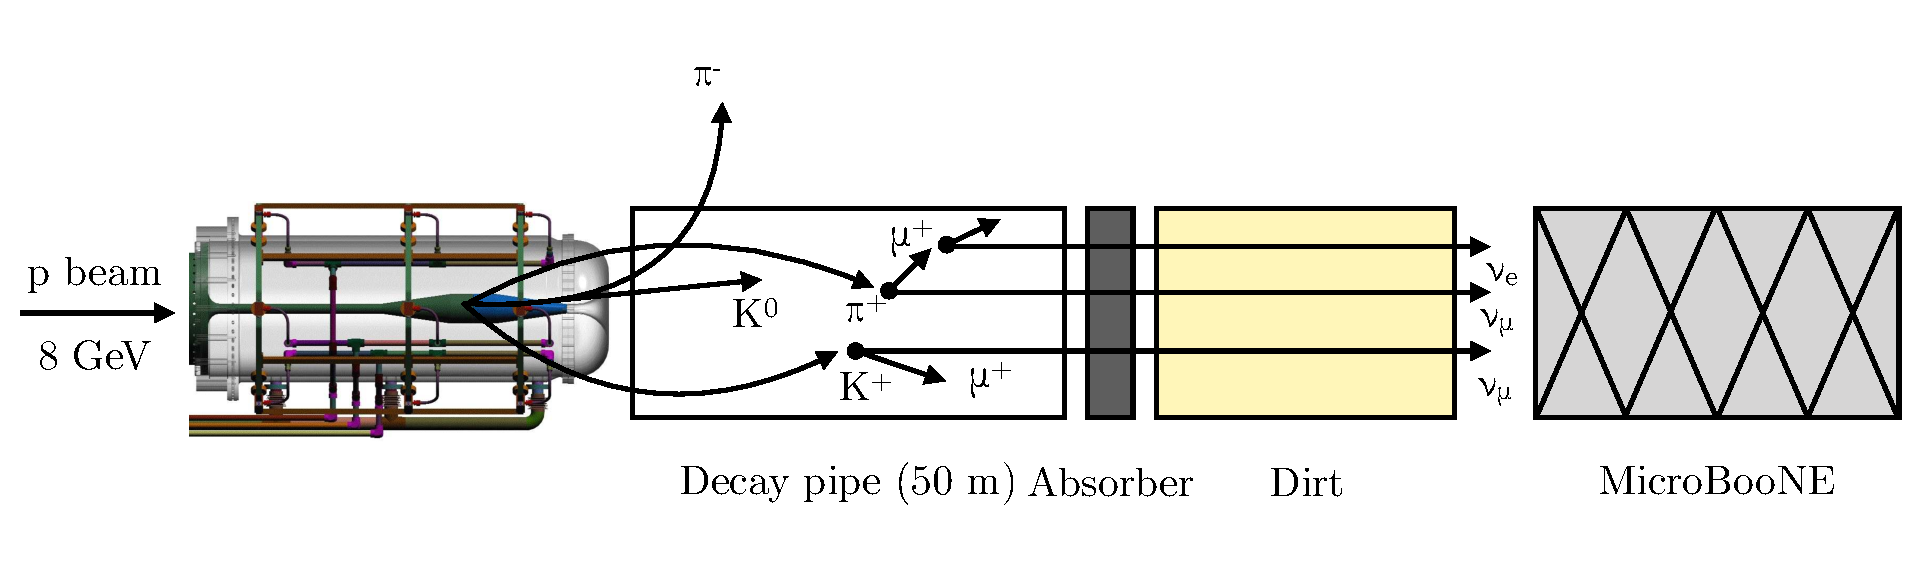
\includegraphics[width=0.98\linewidth]{figures/neutrinobeam.pdf}
    \caption{Schematic of the Booster Neutrino Beam chain in neutrino mode, showing, from left to right, the focusing horn, the decay pipe, the absorber, and the dirt. Dimensions are not to scale.}
    \label{fig:neutrinobeam}
\end{figure}

The hadrons produced in the p-Be interactions are then focused by the electromagnetic horn. The horn is a pulsed toroidal electromagnet with a peak current of 170~kA and a magnetic field at the centre of 1.5~T. It focuses the secondary hadrons along the horn axis: depending on the direction of the current, the positive (negative) charged particles are focused (deflected), producing a neutrino (antineutrino) beam. 

The hadrons with the right charge, mainly kaons and pions, travel through the decay pipe filled with air and are then stopped by a concrete absorber. The neutrinos produced in the decays travel through the ground and hit the detector, which in the case of MicroBooNE is placed 470~m far from the target. Figure \ref{fig:neutrinobeam} shows a schematic of the Booster Neutrino Beam stages in the neutrino mode. 

The muon neutrinos come from the decay of the pions (and in turns of the muons) and the decay of the kaons. Muons and kaons are also responsible for the electron neutrino contamination in the beam. Figure \ref{fig:bnbflux} shows the flavour composition of the BNB flux in neutrino mode at the MicroBooNE location.

\begin{figure}[htbp]
    \centering
    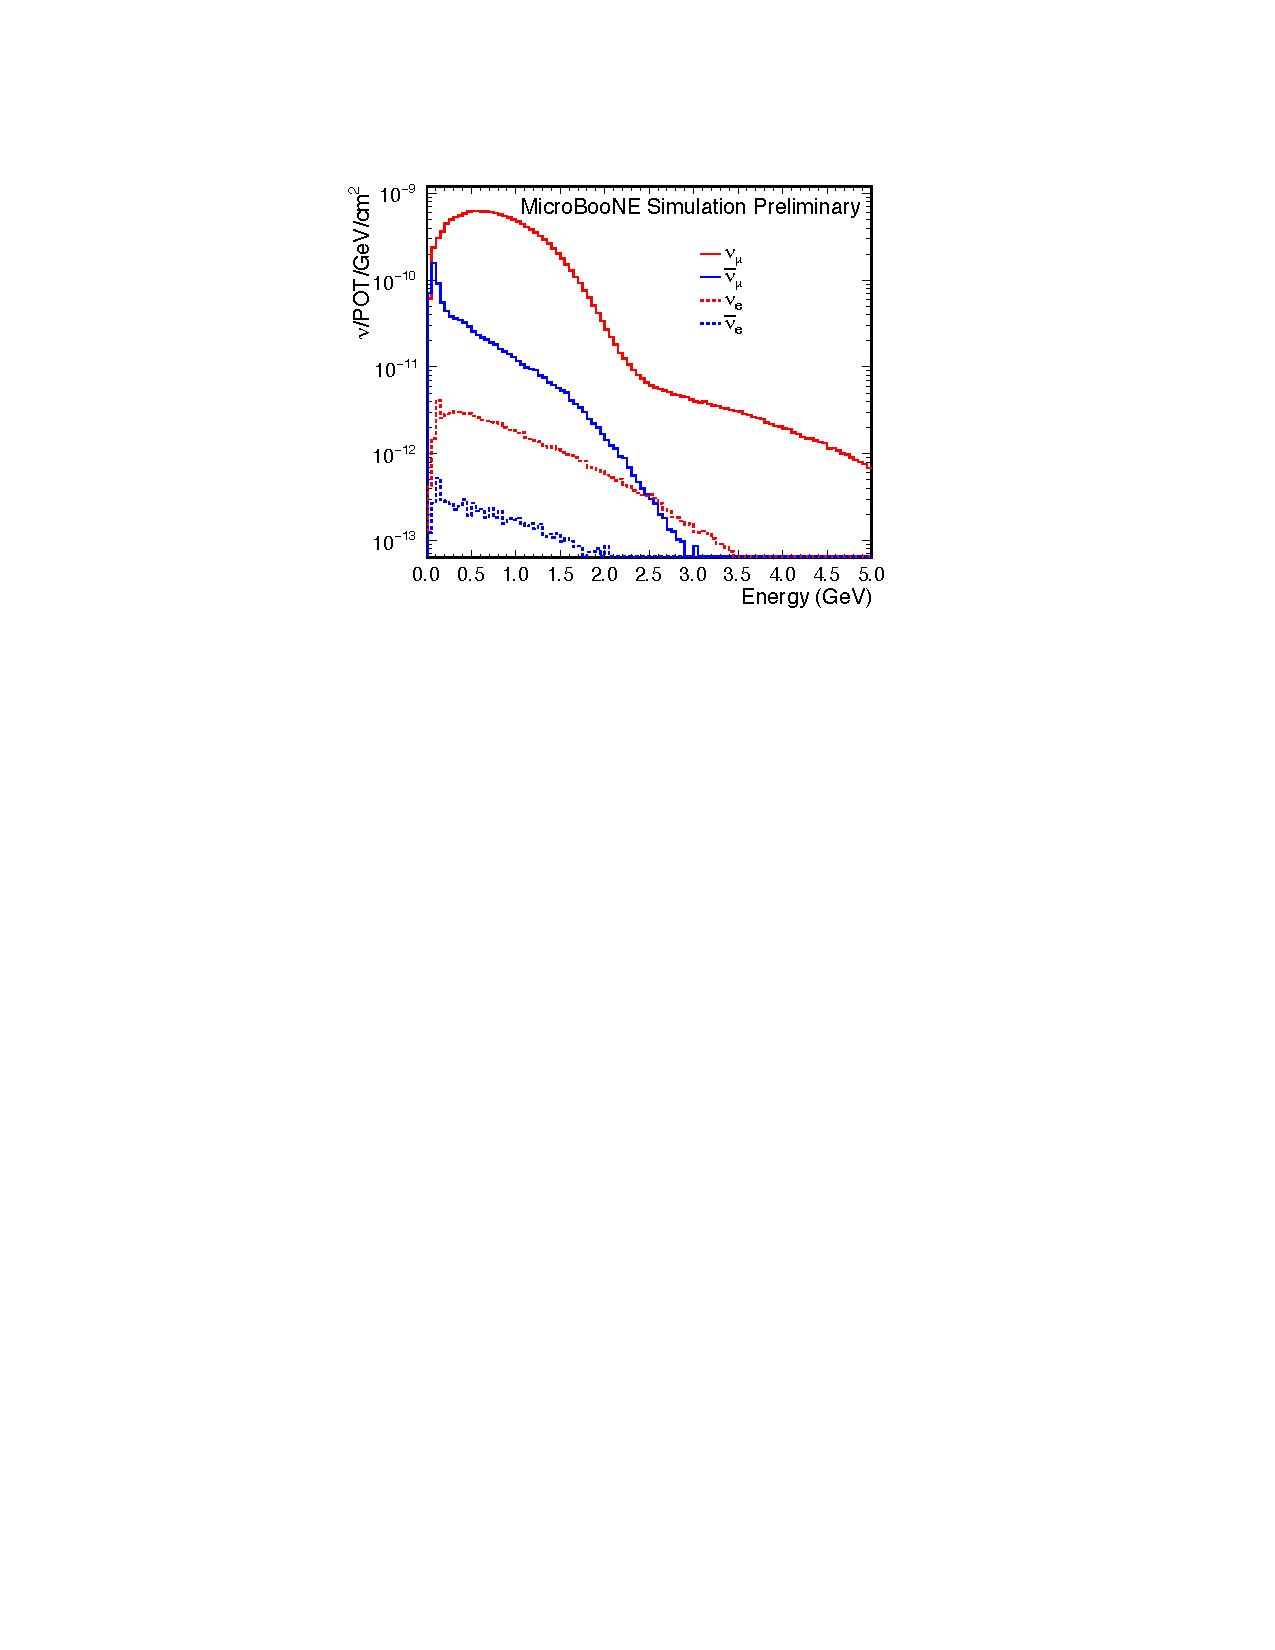
\includegraphics[width=0.7\linewidth]{figures/bnbflux.pdf}
    \caption{BNB absolute flux prediction in neutrino mode at the MicroBooNE location, break down by neutrino flavour.}
    \label{fig:bnbflux}
\end{figure}


The pulsed structure of the neutrino beam is of fundamental importance for on-surface experiments like MiniBooNE and MicroBooNE. In order to suppress non-beam related backgrounds (such as cosmic rays), the detector is triggered only in coincidence with the beam-gate window. In this way, MiniBooNE achieved a cosmic-ray background rejection of 99.987\% \cite{AguilarArevalo:2008qa}. For a LArTPC such as MicroBooNE, the cosmic-ray rejection is more challenging, since the data acquisition window must be at least as long as the drift time window (so in the order of the milliseconds). The techniques employed to reject cosmic rays will be described in Section \ref{sec:methodology}.
 
\subsection{Neutrino flux simulation}\label{sec:flux}
The MiniBooNE collaboration developed a detailed simulation of the BNB flux, described in \cite{AguilarArevalo:2008yp}. 

Here, we will enumerate the main stages of the simulation, in order to clarify the flux systematic uncertainties assessment in Section \ref{sec:systematics}:
\begin{description}
\item[Beamline geometry.] The geometry of the beamline components is simulated in detail, including the beam horn, the target, and the decay pipe. 
\item[Proton generation.] The number of protons delivered by the beam must be precisely estimated, accounting also for beam optics effects.
\item[Interactions of protons with the target.] This is the step with the largest uncertainty. The MiniBooNE collaboration estimated the $\pi^+$ and $\pi^-$ production using the data from the HARP experiment \cite{Catanesi:2005rc}, while the $K^+$ component was constrained using the result of the SciBooNE experiment \cite{Cheng:2011wq}. 
\item[Propagation in the material.] The interaction of the particles in the material is simulated with the GEANT toolkit \cite{Brun:1994aa}.
\item[Particles decay into neutrinos.] The branching ratios and the kinematic properties of the particles which produce the neutrino beam must be assessed with precision.
\end{description}

Table \ref{tab:flux_syst} shows the uncertainties on the various components of the BNB flux for the MicroBooNE experiment. These uncertainties will be reflected in the flux systematic uncertainties of the analysis described in Section \ref{sec:systematics}.

\begin{table}[htbp]
   \centering
     \caption{Systematic uncertainties on the BNB flux calculation. The other category includes uncertainties in pion and nucleon cross-sections on beryllium and aluminium, as well as the horn current calibration uncertainty, and uncertainty in the horn current distribution.}
   \begin{tabular}{p{0.28\linewidth}p{0.1\linewidth}p{0.1\linewidth}p{0.1\linewidth}p{0.1\linewidth}}
     \toprule
     Systematic uncertainty & $\nu_{\mu}/\%$ & $\bar{\nu}_{\mu}/\%$ & $\nu_e/\%$ & $\bar{\nu}_e/\%$ \\
     \midrule
     Proton delivery & 2.0 & 2.0 & 2.0 & 2.0 \\
     $\pi^+$ & 11.7 & 1.0 & 10.7 & 0.03 \\ 
     $\pi^-$ & 0.0 & 11.6 & 0.0 & 3.0 \\
     $K^+$ & 0.2 & 0.1 & 2.0 & 0.1 \\
     $K^-$ & 0.0 & 0.4 & 0.0 & 3.0 \\
     $K^0_L$ & 0.0 & 0.3 & 2.3 & 21.4 \\
     Other & 3.9 & 6.6 & 3.2 & 5.3 \\
     \midrule
     Total & 12.5 & 13.5 & 11.7 & 22.6~\%\\
     \bottomrule
   \end{tabular}
\label{tab:flux_syst}
\end{table}


\section{The MicroBooNE detector}\label{sec:detector}
The MicroBooNE detector consists of a rectangular LArTPC with dimensions of $256~$cm (width) $\times~233~$cm (height) $\times~1037~$cm (length) placed in a cylindrical cryostat. It sits on-axis with the BNB, 470~m far from the neutrino beam target. The mass of liquid argon in the active volume, defined as the portion of the argon encompassed by the TPC, is 89~t. 

\begin{figure}[htbp]
    \centering
    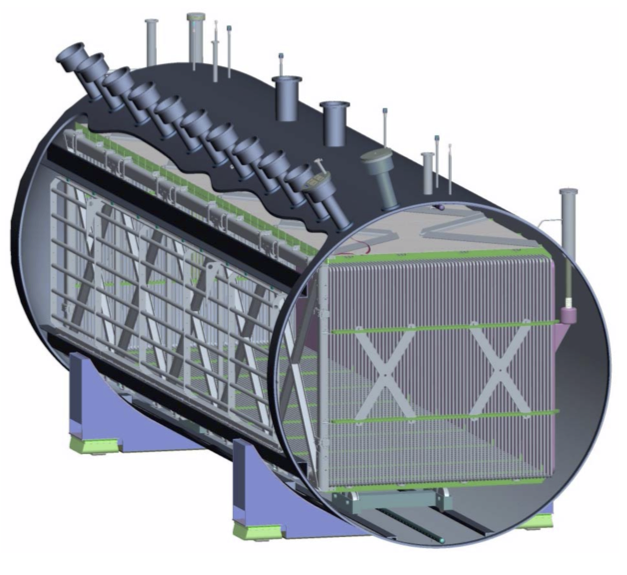
\includegraphics[width=0.7\linewidth]{figures/detector.png}
    \caption{3D rendering of the MicroBooNE cryostat, showing the TPC wire cage and the feedthroughs, which take the signals from the wires and the PMTs (not shown) to the DAQ. In this rendering, the cathode is on the right and the wire planes on the anode side are not shown.}
    \label{fig:detector}
\end{figure}

Figure \ref{fig:detector} shows a 3D rendering of the cryostat containing the TPC. The main components of the detector (the TPC, the light collection system, the cryogenics, the cosmic-ray tagger, and the electronics and readout) are described in detail in \cite{Acciarri:2016smi} and will be summarised below. 

\subsection{The Time Projection Chamber}
The TPC consists of a cathode, an anode, and a field cage. 
%three wire planes with 3 mm spacing at angles of $0^{\circ}$, $+60^{\circ}$, and $-60^{\circ}$ with respect to the vertical. 
The cathode, made of a plane of 9 stainless steel sheets 2.3~mm thick, operates at a voltage of -70~kV.

The field cage, made of 64 stainless steel tubes, creates a uniform electric field of 273~V/cm, stepping down from the -70~kV at the cathode to almost 0~V at the anode, using a resistor chain made of eight 10~M$\Omega$ resistors.

The anode consists of three wire readout planes separated by 3~mm: the drifting electrons induce a bipolar signal in the first two planes (U, V) at $\pm60^{\circ}$ inclination, hence their name \emph{induction planes}, and are then collected by the last plane (Y) at $0^{\circ}$, called \emph{collection plane}, where they produce a unipolar signal. The induction planes are made by 2400 wires, while the collection plane consists of 3456 vertical wires. The wires are separated by a pitch of 3~mm.

The wire planes are held at different voltages (U plane at -110~V, V plane at 0~V, and Y plane at 230~V), in order to minimise the amount of charge collected by the induction planes.

The charge deposited in the TPC generates a signal used to create three distinct two-dimensional views (in terms of wire and time) of the event, which can be combined to reconstruct a three-dimensional image of the interaction. Figure \ref{fig:tpc_coordinates} shows a diagram of the MicroBooNE TPC, with the coordinate system used in the experiment.

\begin{figure}[htbp]
    \centering
    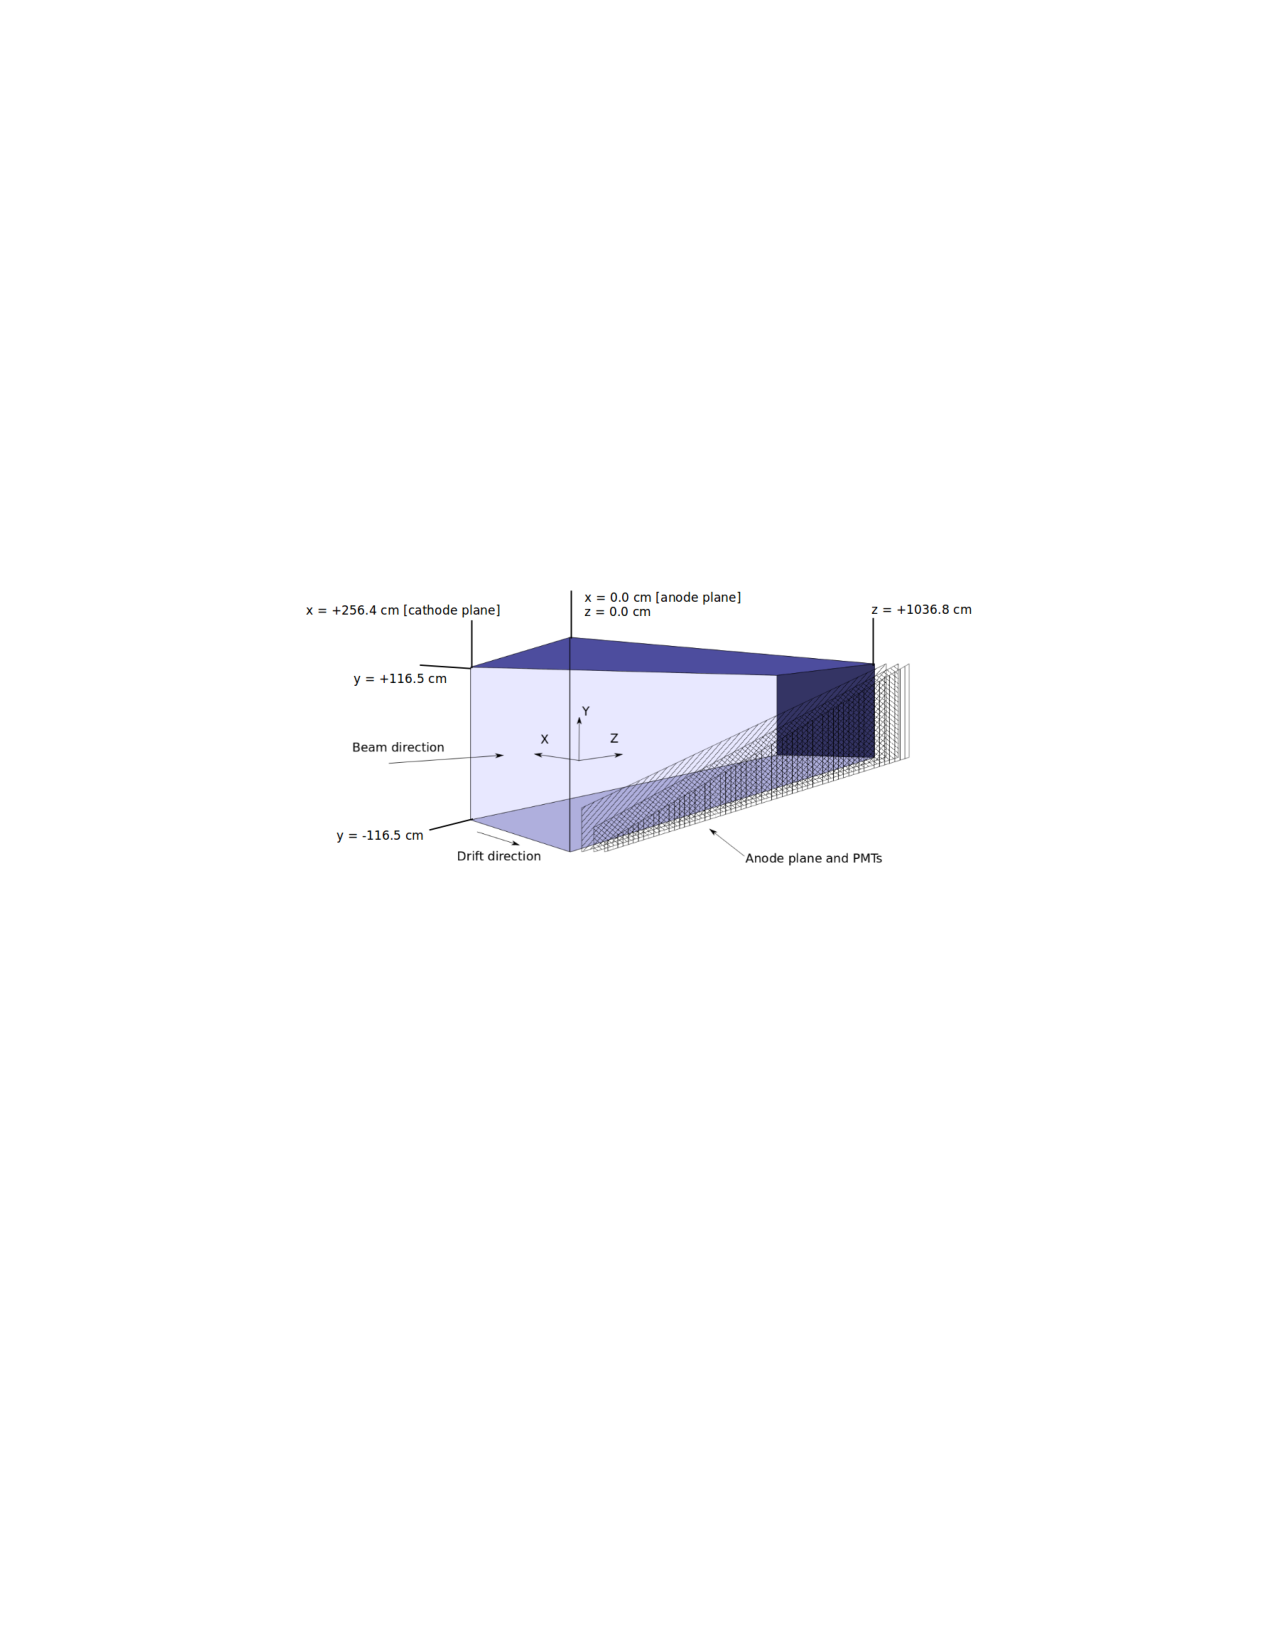
\includegraphics[width=0.95\linewidth]{figures/tpc_coordinates.pdf}
    \caption{Drawing of the MicroBooNE TPC showing the coordinate system and the size of each side. The anode and the cathode are respectively on the right and the left, as seen from the beam.}
    \label{fig:tpc_coordinates}
\end{figure}

MicroBooNE started acquiring neutrino data in October 2015. Figure \ref{fig:evd_ccpi0} shows the event display of a $\nu_{\mu}$ CC$\pi^0$ candidate in the collection plane. The excellent granularity of the detector allows appreciating the electromagnetic showers coming from a $\pi^0\rightarrow\gamma\gamma$ decay and also the small $\delta$-rays produced by the cosmic muons. It is also possible to appreciate the challenge of the pattern recognition, with different topologies and overlapping ionisation trails given by the presence of cosmic rays. 

\begin{figure}[htbp]
    \centering
    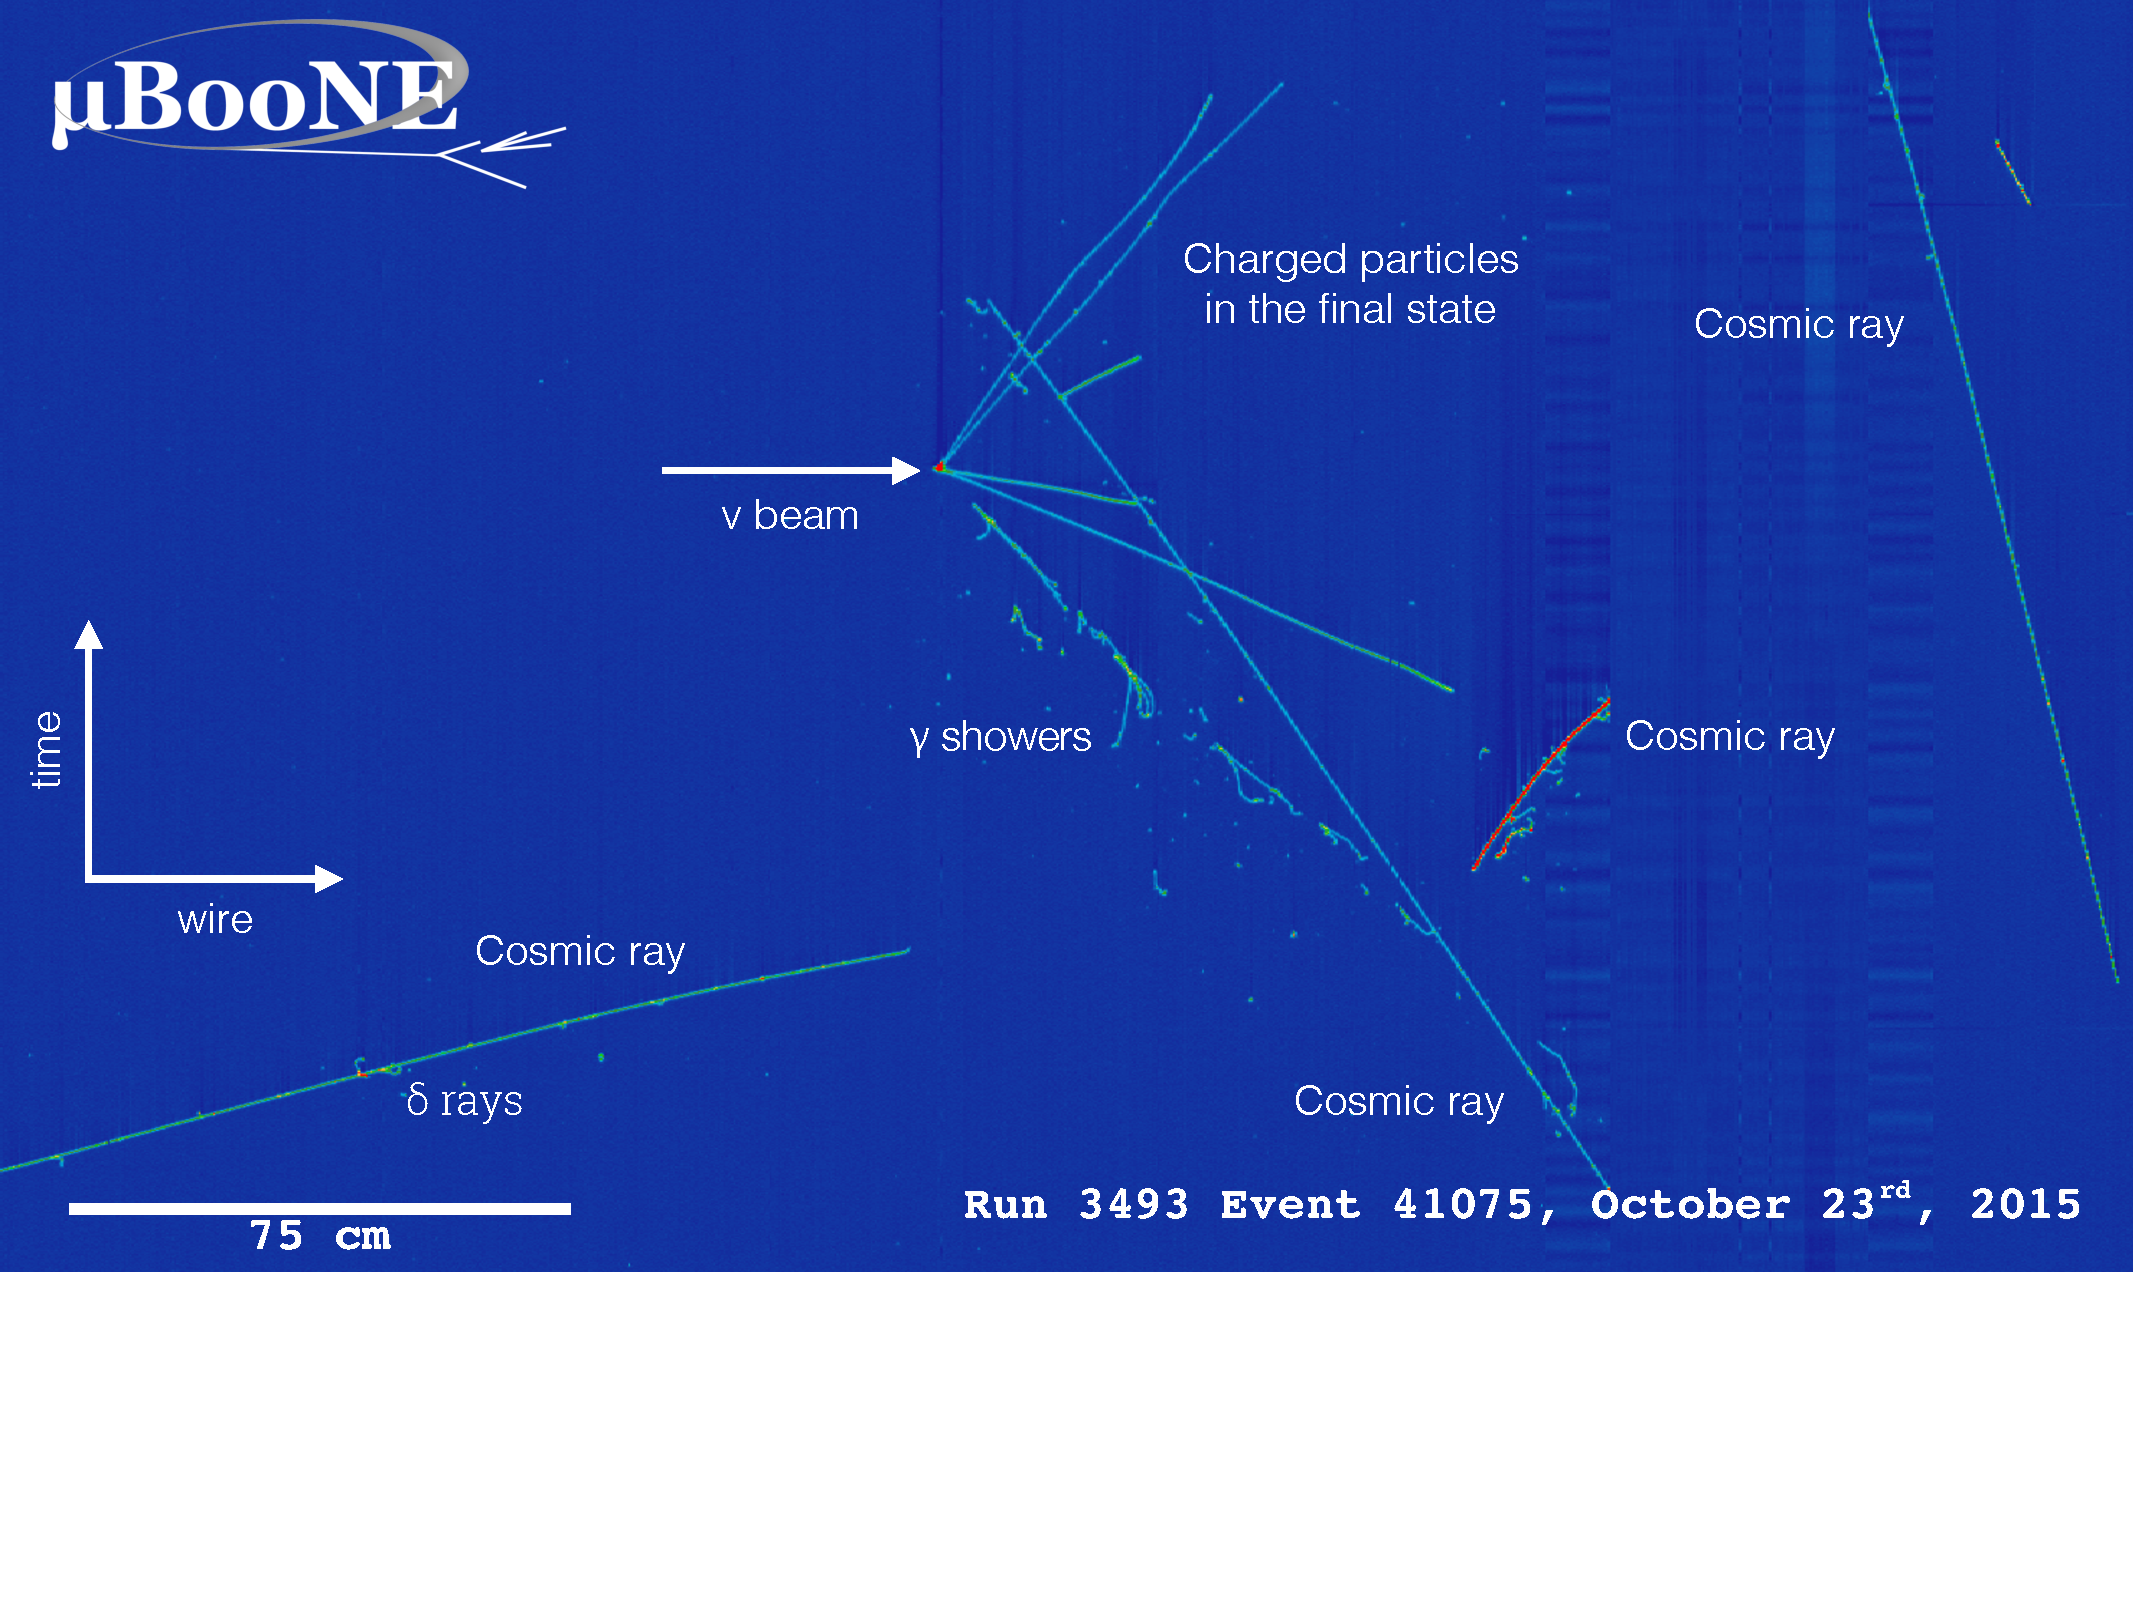
\includegraphics[width=0.9\linewidth]{figures/evd_ccpi0.pdf}
    \caption{Event display of a $\nu_{\mu}$ CC$\pi^0$ candidate in the collection plane. The colour scale corresponds to the amount of charged deposited on the wires.}
    \label{fig:evd_ccpi0}
\end{figure}


\subsection{The Light Collection system}
The MicroBooNE light collection system consists of 32 photomultipliers (PMTs) operating in the liquid argon and placed behind the anode plane, which is 86\% transparent to the light.
The liquid argon scintillation light has a typical spectrum peaked at 128~nm, which must be shifted to a higher wavelength region, where the PMTs have higher efficiency.
MicroBooNE employs tetraphenyl-butadiene (TPB), which absorbs in the UV and emits at $425\pm20$~nm. The efficiency for transmission through PMT borosilicate glass must also be taken into account (around 90\%).
Figure \ref{fig:light} summarises the light emission and absorption in the MicroBooNE light collection system.

\begin{figure}[htbp]
    \centering
    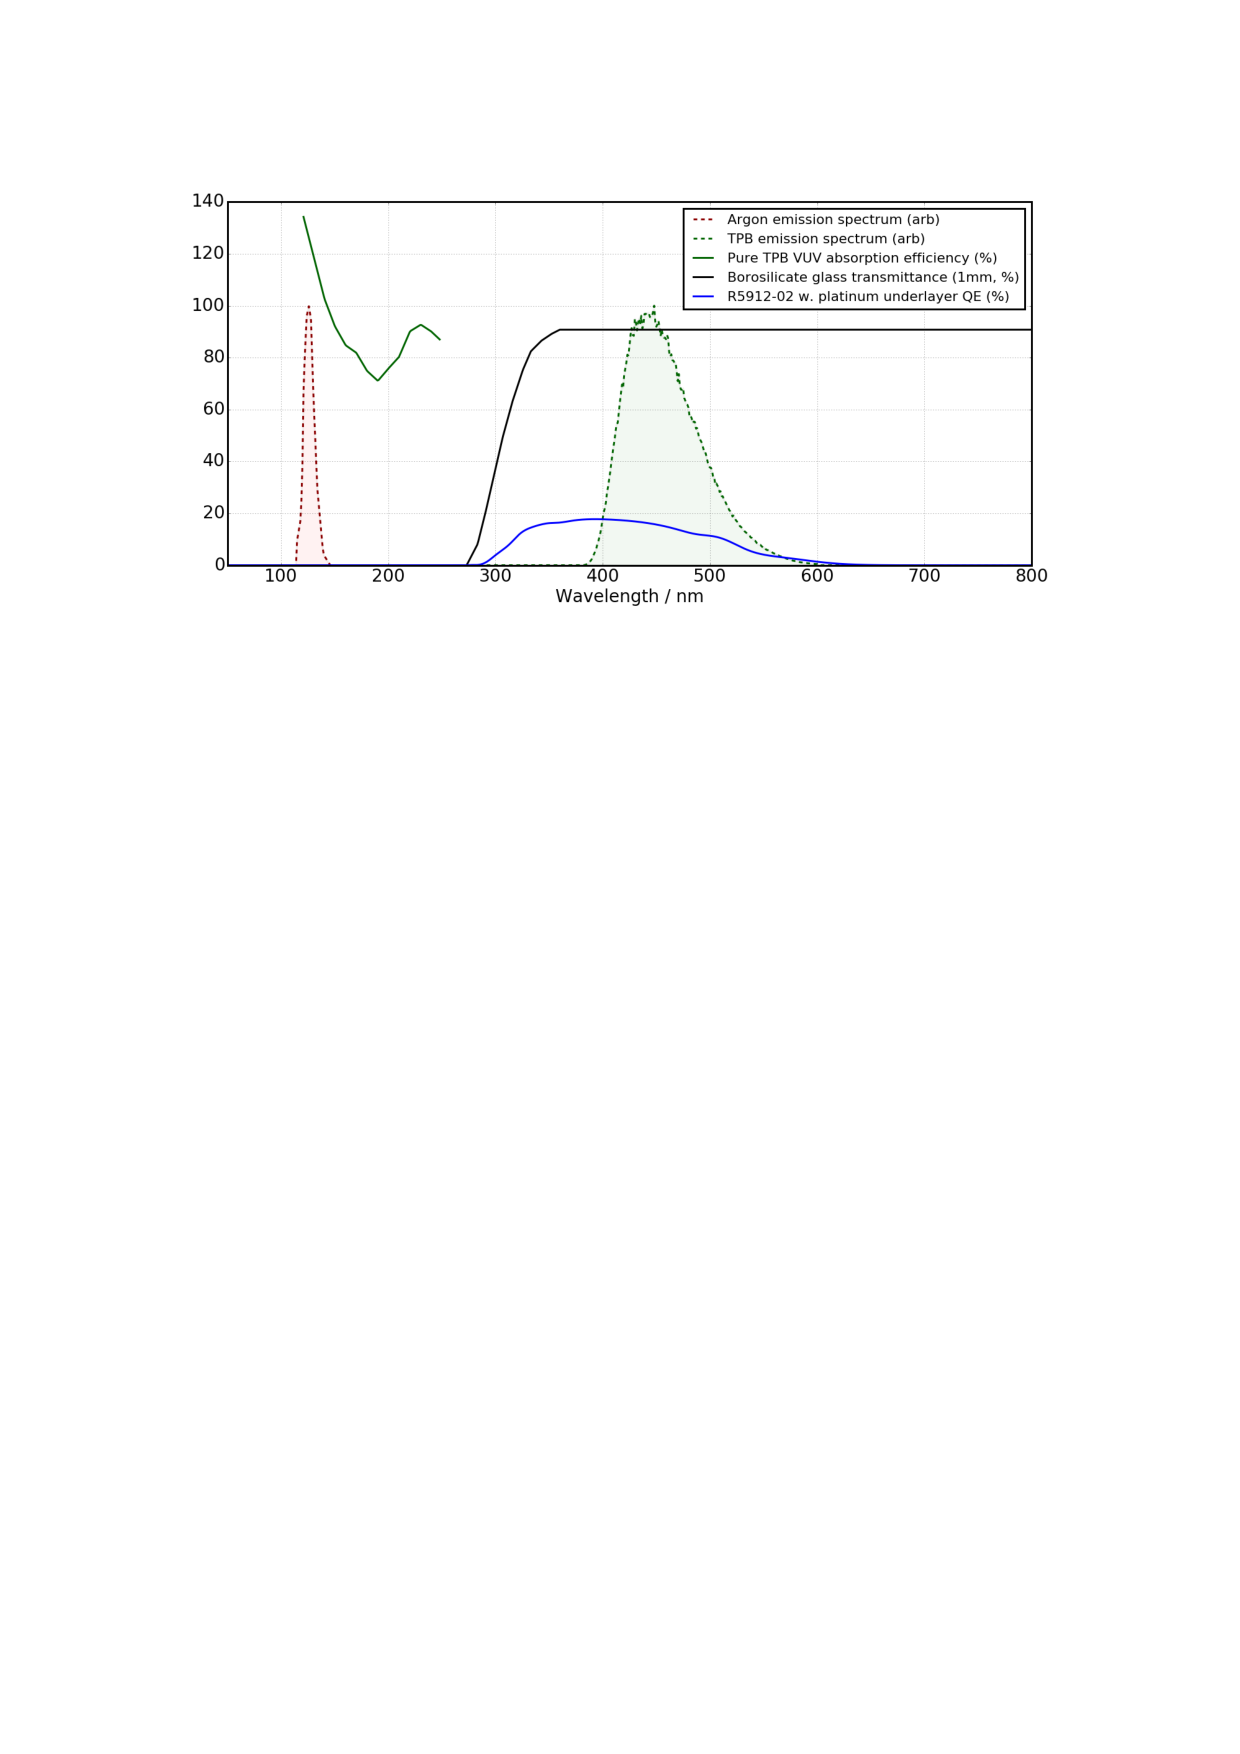
\includegraphics[width=0.85\linewidth]{figures/light.pdf}
    \caption{Scintillation light emission spectrum (red) and TPB re-emission spectrum (green), with the quantum efficiency of the PMTs employed in MicroBooNE (blue). PMT borosilicate glass transmittance is represented by the solid black line. From \cite{Acciarri:2016sli}.}
    \label{fig:light}
\end{figure}

\subsection{Cryogenics and purification}
The liquid argon needs to be kept at a constant temperature and pressure, since they strongly correlate with the drift velocity and, in turn, with the reconstruction of the $x$ coordinate.

The temperature is monitored by 12 Resistive Thermal Devices (RTDs) placed in various location of the cryostat, which is covered with insulating foam to prevent large temperature variations. 

The purification of the liquid argon is performed by a system of two condensers, two pumps, and two filters. The gaseous argon that leaves the detector enters a condenser kept at boiling temperature by liquid nitrogen coils (77~K) and it is then pumped into the filters which mainly remove water and O$_2$ molecules. The performances of the purification system can be quantified by measuring the electron lifetime ratio, as shown in Figure \ref{fig:purity}.

\subsection{Electronics and readout}
MicroBooNE readout electronics can be divided into two main parts: one responsible for the digitisation and recording of the TPC wire signals and one responsible for the digitisation and recording of the PMT signals. 

\paragraph{TPC readout and electronics}
The TPC electronics system can be classified into \emph{cold} electronics, placed inside the cryostat in the liquid argon and responsible for pre-amplification and shaping, and \emph{warm} electronics, placed outside the cryostat and responsible for digitisation and compression of the signals.

The pre-amplification and shaping of the signals happen in the ASIC CMOS chips on cold motherboards placed near the wires, in order to obtain the lowest possible noise. In particular, the wire noise is reduced by a factor of 2 when going from room temperature to liquid argon boiling temperature \cite{Chen:2012kv}. 

The signals are carried through warm wires to the Analog-to-Digital Converters (ADCs) boards and digitised by a 16 MHz clock. The waveforms are then processed in Front-End Modules (FEMs) and down-sampled to 2 MHz. The output consists of time-ordered waveforms of 9600 time-ticks, for a total of 4.8~ms.%, which is three times the drift-time window. 

\paragraph{PMTs readout and electronics}
The signals coming from the 32 PMTs are mainly used in MicroBooNE for the software trigger, as described in Section \ref{sec:trigger}, and to store information on the light emitted by the liquid argon scintillation.

Signals from the PMTs are first split by a dedicated circuit in a high-gain ($\sim20$~ADC/PE) and a low-gain ($\sim2$~ADC/PE) channel which carry 18\% and 1.8\% of the total signal amplitude, respectively.

Then, they are amplified and shaped with a 60~ns rise time and finally digitised at 64 MHz (15.625 ns time-tick). The waveforms are stored over a window of 1500 time-ticks (23.4~\si{\micro}s), starting 4~\si{\micro}s before the beam gate, which is 1.6~\si{\micro}s (10~\si{\micro}s) long for the BNB (NuMI beam). Digitised waveforms outside this window are stored only if above 130 ADC counts (around 6.5~PE) and for a duration of 40 time-ticks (0.6~\si{\micro}s), in order to reduce the data stream. A dead-time of 45 samples (0.7~\si{\micro}s) follows each recorded out-of-beam-gate digitised waveform.



\subsection{The MuCS and the Cosmic-Ray Tagger}\label{sec:crt}

Being located almost on surface, the MicroBooNE detector is constantly subject to a constant $\sim5.5$~kHz cosmic-ray rate \cite{Acciarri:2017rnj}, which corresponds to around 13 cosmic rays for a drift-time window of 2.3~ms. 

In order to study the challenges of cosmic-ray reconstruction, the MicroBooNE detector was also equipped with a small external muon counter stack (MuCS), installed at the start of operations in 2015. 

This sub-detector was used to measure for the first time the cosmic-ray reconstruction efficiency in a LArTPC. This measurement is described in detail in the publication reported in Appendix \ref{sec:mucs}, whose corresponding author is the author of this thesis. Triggering on the signal coming from this small muon counter stack allowed to measure the fraction of cosmic-ray tracks effectively reconstructed in the LArTPC. The measured efficiency is 97.1\%, in agreement with the Monte Carlo simulation. 

This study was also used to demonstrate the tagging capabilities of a larger Cosmic-Ray Tagger (CRT), which surrounds the cryostat on four sides and represents the first cosmic-ray tagging system integrated with a LArTPC \cite{Auger:2016tjc}. Figure \ref{fig:mucs_crt} shows a simulation of the cosmic rays which hit the LArTPC and are tagged by the MuCS and the CRT.

\begin{figure}[htbp]
\centering
  \begin{subfigure}{0.48\textwidth}
    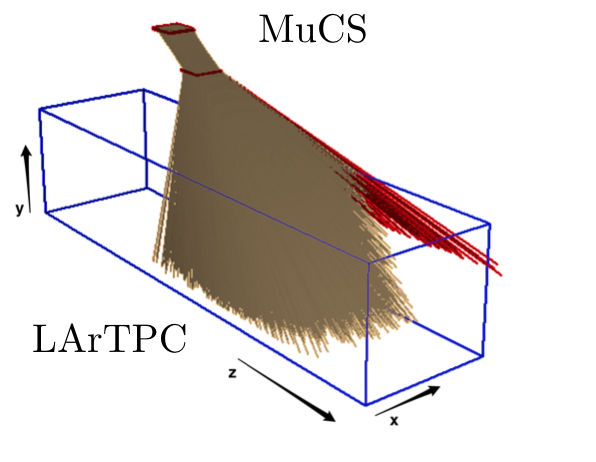
\includegraphics[height=0.7\linewidth]{figures/mucs.png}
    \caption{Cosmic rays hitting the MuCS. Red lines correspond to cosmic rays hitting the MuCS but missing the LArTPC.}
  \end{subfigure}\hfill
  \begin{subfigure}{0.48\textwidth}
    \begin{center}
        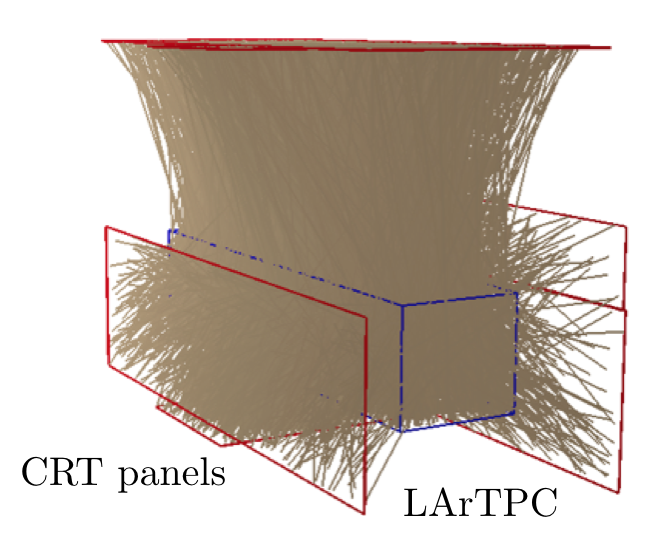
\includegraphics[height=0.7\linewidth]{figures/crt_panels.png}
        \caption{Cosmic rays hitting at least of the one of the CRT panels and the LArTPC.}
    \end{center}
  \end{subfigure}
    \caption{3D drawing of simulated cosmic rays (brown lines) hitting the LArTPC and tagged by the MuCS (left) and the CRT (right).}\label{fig:mucs_crt}
\end{figure}

This sub-system was installed at Fermilab in 2017 and was not present when the data used in this thesis was acquired. 

The CRT panels are made of plastic scintillation modules, which provide time and position information for charged particles crossing the panels and hitting the TPC.
Cosmic-ray rejection in the LArTPC can be improved both by spatially tagging crossing cosmic rays and by vetoing events with a signal in the CRT during the beam-gate window. 

\subsection{Trigger system}\label{sec:trigger}
MicroBooNE employs different triggers in order to minimise the amount of stored data, while keeping a very high neutrino efficiency.

A hardware trigger is fired for each beam spill in the Booster and in the NuMI neutrino beams. When received, a 23.4~\si{\micro}s window is opened in the PMT readout and a 4.8~ms window is opened in the TPC readout. These two triggers (one for the BNB and one for NuMI) have the highest priority, and in case the two beam-gate windows overlap, the precedence is given to the BNB. The beam trigger efficiency is 99.8\%.

Each event in MicroBooNE requires around 30~MB of storage which, for a 5~Hz beam-trigger rate, would correspond to 13~TB/day. However, most beam spills do not produce an effective neutrino interaction in the detector. In order to minimise the number of events containing only cosmic rays, thus reducing the amount of data stored, the beam trigger is required to be in coincidence with a PMT trigger, implemented at software level. In this way, it is possible to achieve a higher level of sophistication and makes the Monte Carlo simulation of the trigger easier. 

\begin{figure}[htbp]
    \centering
    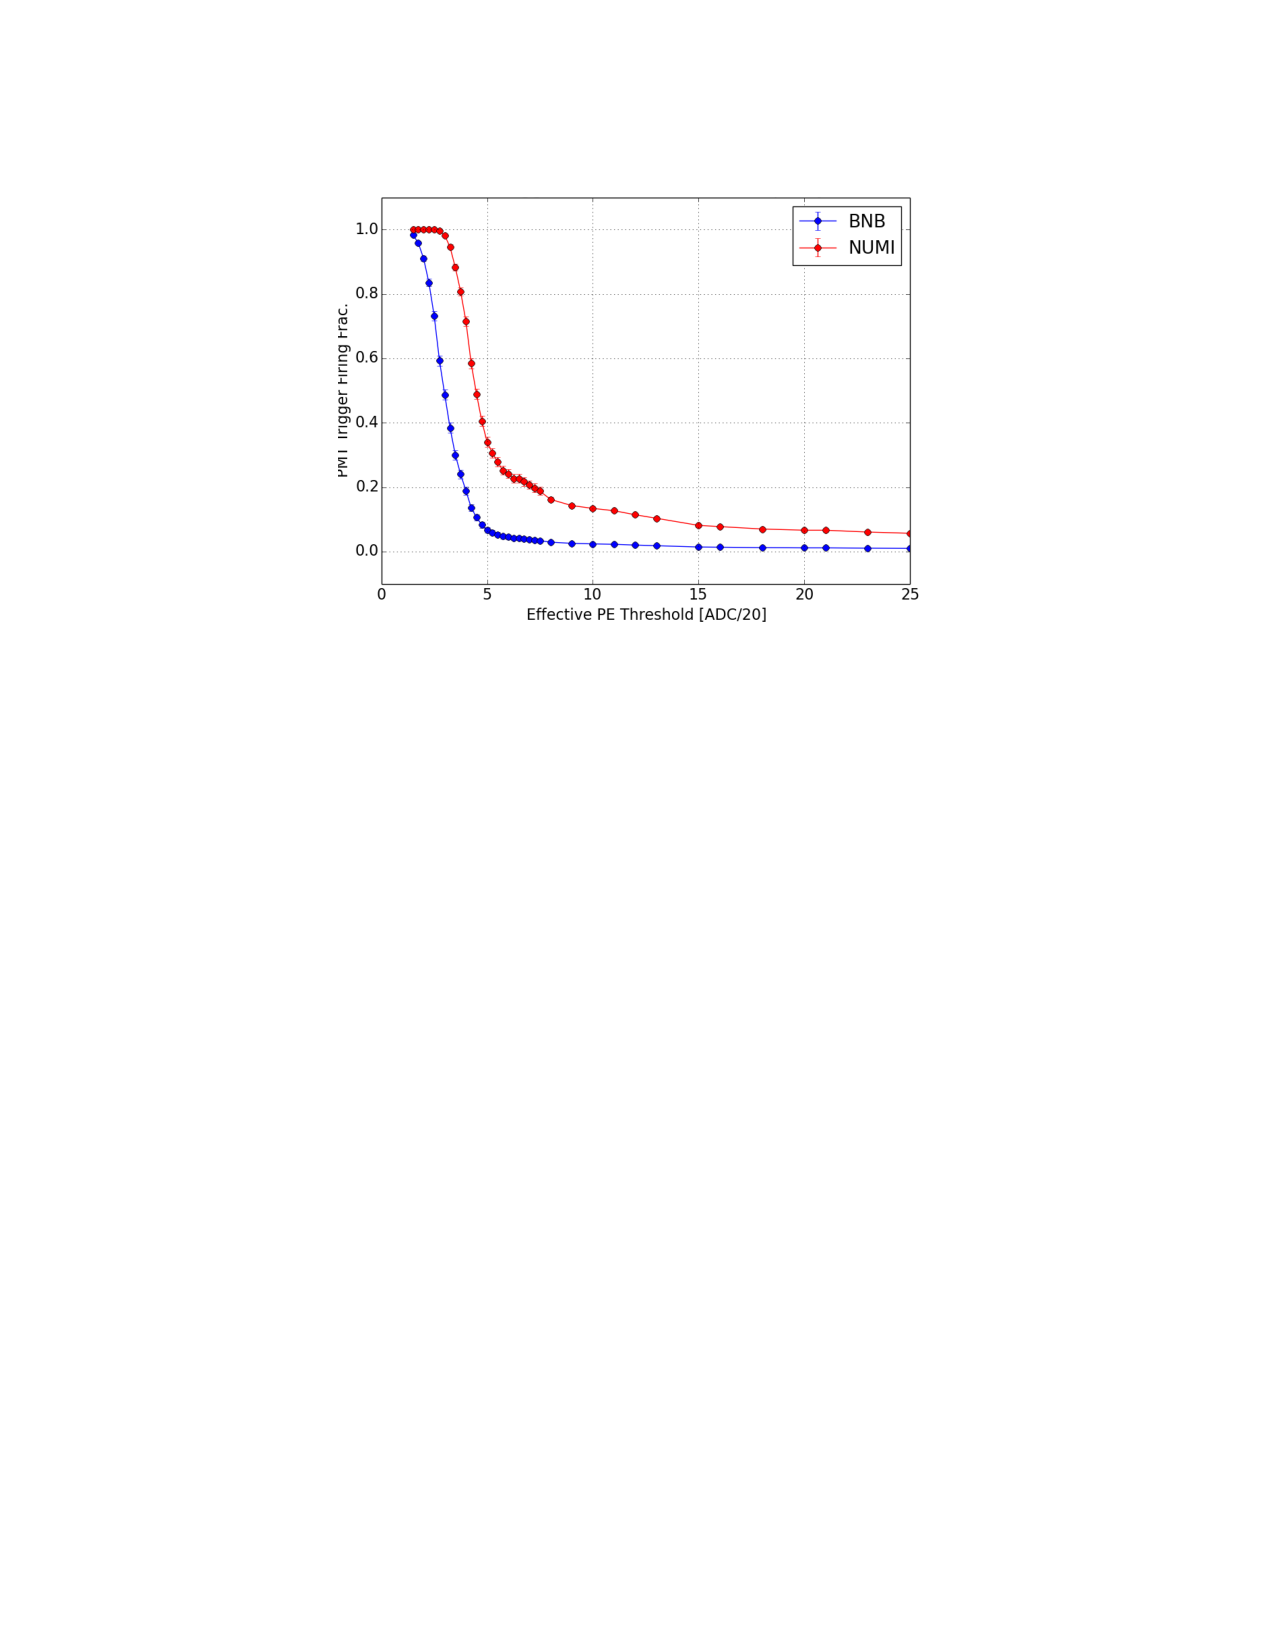
\includegraphics[width=0.85\linewidth]{figures/pmttrigger.pdf}
    \caption{Software trigger efficiency as a function of the PE threshold, both for BNB (blue) and NuMI (red) beam-gate windows.}
    \label{fig:pmttrigger}
\end{figure}

The software trigger requires 6.5 effective PE (photoelectrons) in the light collection system during the beam gate window, rejecting around 97\% of the beam spills. Figure \ref{fig:pmttrigger} shows the software trigger efficiency as a function of the PE threshold, both for BNB and NuMI beam-gate windows.

Cosmic rays can still produce background events if they cross the TPC during the beam gate window, and produce enough scintillation light. In order to precisely assess this background, a trigger, called EXT, is fired at a 0.1~Hz rate orthogonally to the beam-gate windows, requiring 6.5 PE in a 1.6~\si{\micro}s time window (same as the BNB beam trigger). Events selected by this \emph{beam-off} trigger will then contain only cosmic rays.

Figure \ref{fig:trigger} shows the time-distribution of \emph{optical flashes} recorded from events triggered during the BNB beam-gate window. An optical flash is a group of light pulses recorded by the PMTs within a 100~ns time difference. The excess of events corresponds to the 1.6~\si{\micro}s beam spill width. 

\begin{figure}[htbp]
    \centering
    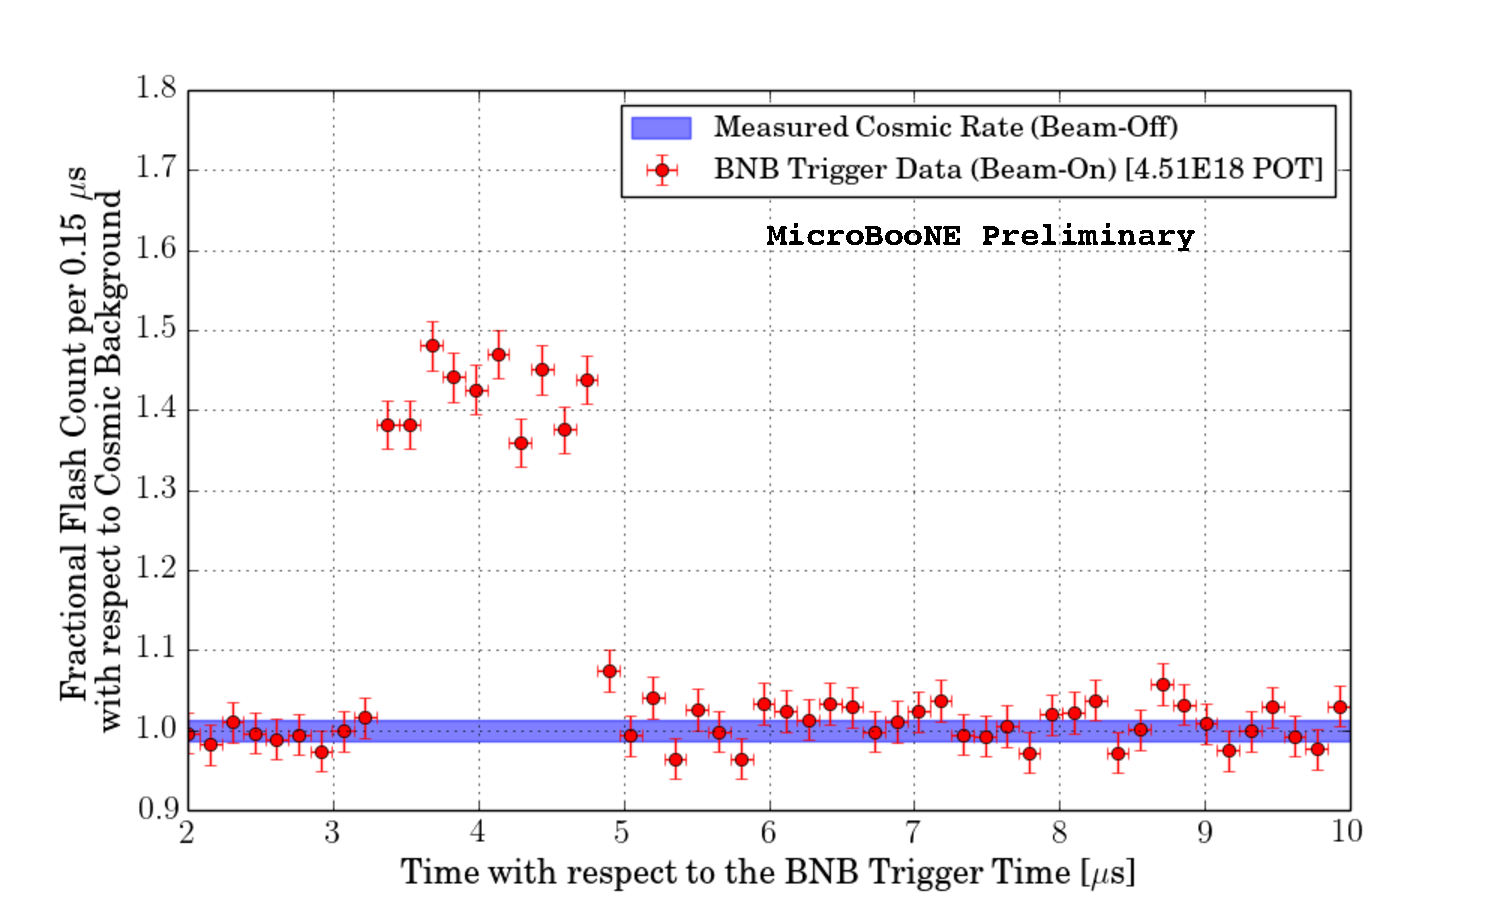
\includegraphics[width=0.85\linewidth]{figures/trigger.pdf}
    \caption{Distribution of optical flash times with respect to the trigger time for BNB triggered events, shown as a ratio to the expected cosmic rate from beam-off data, collected with the EXT trigger.}
    \label{fig:trigger}
\end{figure}

The DAQ (data acquisition) system takes as input the triggered TPC and PMT readouts and translates the raw data format into ROOT files, one for each trigger. As of January 2019, MicroBooNE has collected $1.2\times10^{21}$ POT in BNB neutrino mode, which roughly corresponds to the amount of POT collected by MiniBooNE (which collected also $1.1\times10^{21}$ POT in antineutrino mode and $1.9\times10^{20}$ POT in beam dump mode).
This document will focus on $4.34\times10^{19}$ POT collected with the BNB trigger between February 23 and May 22, 2016, which corresponds to MicroBooNE \emph{open data sample}. 